\documentclass[master=ecws,masteroption=ss,english]{kulemt}
\setup
    { title={Implementation of Functional Dependencies}
    , author={Michiel Derhaeg}
    , promotor={Prof.\,dr.\,ir.\ Tom Schrijvers}
    , assessor={Dr.\, ir.\, Georgios Karachalias \and Prof.\, dr.\, Bart Jacobs}
    , assistant={Dr.\, ir.\, Georgios Karachalias}
    , acyear={2017 - 2018}
    , inputenc={utf8}
    , translatedtitle={Implementatie van Functional Dependencies}
    , udc={placeholder}
    , shortabstract={short abstract placeholder}
    , inputenc={utf8}
    }
\usepackage{pdfpages}
\usepackage{lmodern}
\usepackage{amssymb,amsmath}
\usepackage{amstext}
\usepackage{cite}
\usepackage{xcolor}
\usepackage{mathpartir}
\usepackage{listings}
\usepackage{ifxetex,ifluatex}
\usepackage{fixltx2e} % provides \textsubscript
\ifnum 0\ifxetex 1\fi\ifluatex 1\fi=0 % if pdftex
  \usepackage[T1]{fontenc}
\else % if luatex or xelatex
  \ifxetex
    \usepackage{mathspec}
  \else
    \usepackage{fontspec}
  \fi
  \defaultfontfeatures{Ligatures=TeX,Scale=MatchLowercase}
\fi
% use upquote if available, for straight quotes in verbatim environments
\IfFileExists{upquote.sty}{\usepackage{upquote}}{}
% use microtype if available
\IfFileExists{microtype.sty}{%
\usepackage[]{microtype}
\UseMicrotypeSet[protrusion]{basicmath} % disable protrusion for tt fonts
}{}
\PassOptionsToPackage{hyphens}{url} % url is loaded by hyperref
\usepackage[unicode=true]{hyperref}
\hypersetup{
            pdfborder={0 0 0},
            breaklinks=true}
\urlstyle{same}  % don't use monospace font for urls
\IfFileExists{parskip.sty}{%
\usepackage{parskip}
}{% else
\setlength{\parindent}{0pt}
\setlength{\parskip}{6pt plus 2pt minus 1pt}
}
\setlength{\emergencystretch}{3em}  % prevent overfull lines
\providecommand{\tightlist}{%
  \setlength{\itemsep}{0pt}\setlength{\parskip}{0pt}}
\setcounter{secnumdepth}{0}
% Redefines (sub)paragraphs to behave more like sections
\ifx\paragraph\undefined\else
\let\oldparagraph\paragraph
\renewcommand{\paragraph}[1]{\oldparagraph{#1}\mbox{}}
\fi
\ifx\subparagraph\undefined\else
\let\oldsubparagraph\subparagraph
\renewcommand{\subparagraph}[1]{\oldsubparagraph{#1}\mbox{}}
\fi
\newcommand{\highlight}[1]{%
  \colorbox{gray!30}{$\displaystyle#1$}}
\newcommand{\fctrans}{\mathbin{\raise 0.6ex\hbox{\oalign{\hfil$\scriptscriptstyle \mathrm{o}$\hfil\cr\hfil$\scriptscriptstyle\mathrm{9}$\hfil}}}}

\newcommand{\guard}{\qquad \mid}
\newcommand{\where}{\qquad \text{where} \;}
\newcommand{\whereindent}{\qquad\qquad\;\;\;}
\newcommand{\systemfc}{System $\text{F}_\text{C}\;$}

% set default figure placement to htbp
\makeatletter
\def\fps@figure{htbp}
\makeatother

\newcommand{\george}[1]{\begin{color}{red}{George says: {#1}}\end{color}}


\begin{document}

\begin{preface}
preface placeholder
\end{preface}

\tableofcontents*

\begin{abstract}
abstract placeholder
\end{abstract}

\listoffigures

\mainmatter

% Introduction
% vim:ft=tex
\chapter{Introduction}
\label{cha:intro}
Type classes were introduced by Wadler and Blott~\cite{Wadler:1989:MAP:75277.75283}
as a
way to express ad-hoc polymorphism, and they have become an essential part of the Haskell
programming language. This feature was quickly extended to allow for multiple
type parameters. Type classes originally allowed us to express properties of a
collection of types and now relations between types as well. Unfortunately, by using
multi-parameter type classes, situations can easily arise where the type
of one or several parameters can not be determined unambiguously. To resolve
these ambiguities, Mark P. Jones introduced the notion of Functional Dependencies
\cite{Jones00typeclasses} between the type parameters of type classes, so one
would be uniquely determined by the other and the ambiguities would be resolved.
It is a technique that originated from relational database theory but applied to
the design of type systems. It became a very popular type system feature that is
used to date. Not just to resolve ambiguities, but also for the
static enforcement of semantic properties and type-level programming.

However, the implementation of this feature in GHC proved to be problematic and
does not behave according to the specification.  Some programs that are entirely
correct
would be rejected by GHC's type checker because at the time it seemed to be
impossible to translate the typing relation into System
F~\cite{systemf},
a polymorphic
lambda calculus often used by functional programming language compilers as an
intermediate representation. No implementation uses pure System F to encode
their source language. It is usually extended to make the translation more
straightforward, readable or simply to support more advanced features. For
example, algebraic datatypes are a common addition. In GHC specifically, the intermediate language has been extended
with support for GADTs~\cite{PeytonJones06}, which seemed over-sophisticated extension to an
intermediate representation at the time. Motivated by
keeping the intermediate language as simple as possible, it was never extended
to support Functional Dependencies and its implementation remained incomplete.

To support features like type
families~\cite{AssociatedTypeSynonyms}, it was proposed by
Sulzmann et al. \cite{Sulzmann:2007:SFT:1190315.1190324} to extend System F with
type equality coercions. This calculus is called System $F_C$ and currently used by
GHC as the new intermediate representation. This new extension is expressive
enough to express most of the more advanced type system features.

Despite the continued popularity of Functional Dependencies it was never
investigated if they could be implemented using the new representation until
recently. Karachalias and Schrijvers \cite{Karachalias:2017:EFD:3156695.3122966}
described a type inference algorithm for functional dependencies and a way to
translate them into System $F_C$.


% Background
\section{Type Classes}
In this section we'll informally describe type classes and their semantics. In the
following example we defined a type class for testing the equality of values
called \texttt{Eq}:

\begin{verbatim}
    class Eq a where
      (==) :: a -> a -> Bool
\end{verbatim}

As we mentioned earlier, type classes allow for ad-hoc polymorphism and the method
specified in the class declaration body can be used with any type that
implements the required methods of the type class by providing an instance.
This differs from parametric polymorphism in the way that the \texttt{(==)}
operator cannot be applied to any type \texttt{a}, but only the types that provide an
instance for the type class. The signature is therefore not entirely honest and
has a implied type class constraint:
\begin{verbatim}
    (==) :: Eq a => a -> a -> Bool
\end{verbatim}
Type signatures that contain type class constraints like the one above are called
\textit{qualified types}~\george{citation here} and could possibly appear in the type signatures of the
functions where these polymophic methods are used.
% TODO example of usage?

To use these polymophic methods we provide an instance declaration for every type
we wish to use them on. The following is an example of a type class instance
delcaration for the \texttt{Bool} type which contains an implementation of the
methods for which a type signature was specified in the corresponding class
declaration.
\begin{verbatim}
    instance Eq Bool where
      True  == True  = True
      False == False = True
      _     == _     = False
\end{verbatim}

A instance declaration for polymorphic types (types with type parameters) might
require certain instance delcarations for these parametrized types. In order to avoid unneccessarily restricting such instances,
we can specify required class constraints in the {\em instance context} of an instance declaration:
\begin{verbatim}
    instance Eq a => Eq [a] where
      []     == []     = True
      (a:as) == (b:bs) = a == b && as == bs
      _      == _      = False
\end{verbatim}
It is required that the equality is also defined for the element type to
implement the equality for lists. Hence, the implication \texttt{Eq a => Eq [a]}
tells us that if we have a instance of \texttt{Eq} for a type \texttt{a}, we
automatically also have an instance for a list of \texttt{a}s

The next example is a class declaration of the \texttt{Ord} type class, which
represents ordering. The implication in the declaration specifies a hierarchy
between type classes. This means that providing an instance declaration for the
\textbf{superclass}, in this case \texttt{Eq}, is a prerequisite for being
able to define an instance declaration for \texttt{Ord}.

Note that the implication should be interpreted in the inverse direction and
actually means: if we have a instance for \texttt{Ord} we also have one for
\texttt{Eq}.
\begin{verbatim}
    class Eq a => Ord a where
      (<=) :: a -> a -> Bool
\end{verbatim}

Type classes could be extended to not just support one type parameter but
multiple parameters and we can define functional dependencies between these
types. These concepts will be described in the next section.

\section{Functional Dependencies}
% syntax
% examples
\begin{verbatim}
class Collection c e where
    singleton :: e -> c
\end{verbatim}

\begin{verbatim}
class Collection c e | c -> e where
    singleton :: e -> c
\end{verbatim}

\begin{verbatim}
instance Collection [a] a where
    singleton x = [x]
\end{verbatim}

\begin{verbatim}
instance Collection ByteArray Byte
instance Collection ByteArray Bit
\end{verbatim}

\begin{verbatim}
singleton2 :: (Singleton c2 c1, Collection c1 e) => e => c2
singleton2 e = singleton (singleton e)
\end{verbatim}
% semantics

% vim:ft=tex
\section{Problem Statement}
\label{sec:problem-statement}
Despite the popularity of functional dependencies, the feature remains unreliably
implemented in GHC. Due to the lack expressiveness of the previous intermediate
representation based on System F, it is impossible to elaborate (translate)
Haskell programs that are entirely correct (well-typed and perfectly valid
according to the specification) in GHC and are thus rejected by GHC's type checker.

The following example illustrates such a case where GHC would reject a perfectly
valid program.
\begin{verbatim}
    class C a b | a -> b
    instance C Int Bool

    f :: C Int b => b -> Bool
    f x = x
\end{verbatim}

\texttt{f} is a function that simply returns its argument but has a rather
exotic type signature. It contains a polymorphic type \texttt{b} and a type
class constraint for \texttt{C Int b}. Due to the functional dependency in the
class declaration of \texttt{C}, we know that \texttt{b} in the type class
constraint could only have one possible type: \texttt{Bool}. This can be
derived from the instance declaration. \texttt{b} should therefore always be
equal to \texttt{Bool}. This means that this program is well-typed and perfectly
valid. Despite that this program is entirely correct, the relationship between
\texttt{Int} and \texttt{Bool} can not be translated into System F.

When support for type families and associated types was added to GHC, the
intermediate representation was extended to support type level functions similar
to type families and explicit type equality coercions~\cite{Sulzmann:2007:SFT:1190315.1190324}. This new representation
is called System $F_C$. Instead of it being another ad-hoc extension, it was a
more general and powerful solution that could host a multitude of existing and
future type system features, e.g. GADTs, while remaining relatively simple
and straightforward to translate to.

The new representation features explicit type equality coercions, proofs that
could be constructed by the compiler, that witness type equalities. These
coercions can be used to explicitly and safely type cast expressions.

The possibility of implementing functional dependencies by elaborating them into
System $F_C$ was not fully explored any further until recently. Karachalias and
Schrijvers\cite{Karachalias:2017:EFD:3156695.3122966} presented a type
inference algorithm for functional dependencies and a way to elaborate them into
System $F_C$.

This thesis will present a fully functional implementation of the aforementioned
algorithm and a description of important implementation-specific details and
complications that may arise throughout the development of this implementation.

Eventually, this implementation is not only aiming to implement support for functional dependencies,
but GADTs and type families as well. So the interaction between these features
and their implementations can be studied. Especially conflicts and complications
that may arise during the development of all these features might be very
interesting.

Firstly, this implementation will serve as a validation of the specification
that might reveal potential inaccuracies. And secondly, as a feasibility study
that shows that it is possible to fully implement functional dependencies by
reusing the available framework that is currently in place in GHC.


% System Fc
\section{System $F_C$}

In this section we'll define and discuss System $F_C$, the new target language
of the compiler. It is extended from System F in a few ways that makes it able
to support a multitude of more advanced source-language type system features
like Type Families, Generalised Algebraic Datatypes, and most relevant to us,
Functional Dependencies.

System $F_C$ extends polymorphic lambda calculus with explicit type equality
witnesses, or proofs, called coercions. And with type-level functions and
top-level axioms which are their instantiations.

% Discuss other additions other additions to System F like datatypes

\subsection{Syntax}

%TODO highlight new stuff
\begin{figure}
\begin{align*}
    v &::= a \;  \; | \;  \; T \;  \; | \;  \; v_1 \;  \; | \;  \; v_2  \; | \;
    \highlight{F(\overline{v})}  \; | \;  \forall a. v  \; | \; \highlight{\psi
    \Rightarrow v} &\textit{Types}\\ \\
    \highlight{\gamma} &::= \highlight{\langle v \rangle \; | \; \text{sym} \; \gamma \; | \;
    \text{left} \; \gamma \; | \; \text{right} \; \gamma \; | \; \gamma_1 ;
    \gamma_2 \; | \; \psi \Rightarrow \gamma} &\textit{Coercions} \\ 
    \; &\quad \highlight{| \; \; F(\overline{\gamma}) \; | \; \forall a . \; \gamma \; | \;
    \gamma_1 [\gamma_2] \; | \; g \; \overline{v} \; | \; c \; | \; \gamma_1 @
    \gamma_2 \; | \; \gamma_1 \; \gamma_2} \\ \\
    \highlight{\psi} &::= \highlight{v_1 \sim v_2} &\textit{Propositions}\\ \\
    t &::= x \; | \; K \; | \; \Lambda a . \; t \; | \; t \; v \; | \;
    \lambda(x\; : \; v). \; t \; | \; t_1 \; t_2 \; | \; \highlight{\Lambda(c \; : \psi).
    \; t} &\textit{Terms} \\
          &\quad | \; \; t \; \gamma \; | \; \highlight{t \triangleright \gamma} \; | \;
    \textbf{case} \; t_1 \; \textbf{of} \; p \rightarrow t_2 \; | \;
    \textbf{let} \; x : v = t_1 \; \textbf{in} \; t_2 \\ \\
    p &::= K \; \highlight{\overline{b} \; (\overline{c : \psi})} \; (\overline{d : \tau})
    \; (\overline{f : v}) &\textit{Patterns}\\ \\
    decl &::= \textbf{data} \; T \; \overline{a} \; \textbf{where} \; K : v
         &\textit{Declarations}\\
         &\quad | \; \; \textbf{let} \; x : v = t \\
         &\quad | \; \; \highlight{\textbf{type} \; F(\overline{a})} \\
         &\quad | \; \; \highlight{\textbf{axiom} \; g \; \overline{a} :
         F(\overline{u}) \sim \; v} \\
\end{align*}
\caption{System $F_C$ syntax}
\label{fc-syntax}
\end{figure}

The highlighted parts are the things that are different from standard System F.

\subsubsection{Type equality coercions}

Coercions, denoted by $\gamma$, are the main interesting addition to the target
language. These are proofs which are usually constructed during the elaboration
of the source language. These coercions can then be used during typechecking to
explicitly cast a term $e : v_1$ to type $v_2$ if a coercion is provided that
witnesses the equality between these types.

\subsubsection{Type functions}

\subsection{Typing}
% TODO other typing rules
\begin{figure}[h]
% TERM
$$
%TmCast
\inferrule*[right=TmCast]
{P;\Gamma \vdash_{tm} t : v_1 \\ P;\Gamma \vdash_{co} \gamma : v_1 \sim v_2}
{P;\Gamma \vdash_{tm} t \triangleright \gamma : v_2}
$$
$$
%TmVar
\inferrule*[right=TmVar]
{x : v \in \Gamma}
{\Gamma \vdash_{tm} x : v}
$$
$$
%TmCon
\inferrule*[right=TmCon]
{K : v \in \Gamma}
{\Gamma \vdash_{tm} K : v}
$$
$$
%TmAbs
\inferrule*[right=TmAbs]
{x \notin dom(\Gamma) \qquad \Gamma \vdash_{ty} v_1 : \star \qquad \Gamma , x : v_1
\vdash_{tm} t : v_2}
{\Gamma \vdash_{tm} \lambda(x : v_1). t : v_1 \rightarrow v_2}
$$
$$
%TmApp
\inferrule*[right=TmApp]
{\Gamma \vdash_{tm} t_1 : v_2 \rightarrow v_1 \qquad \Gamma \vdash_{tm} t_2 : v_2 }
{\Gamma \vdash_{tm} t_1 \; t_2 : v_1}
$$
$$
%TmTyApp
\inferrule*[right=TmTyApp]
{\Gamma \vdash_{tm} t : \forall (a : k). v \qquad \Gamma \vdash_{ty} v_1 : k}
{\Gamma \vdash_{tm} t \; v_1 : [a \mapsto v_1]v}
$$
$$
%TmTyAbs
\inferrule*[right=TmTyAbs]
{a \notin dom(\Gamma) \\ \Gamma , a : k \vdash_{tm} t : v}
{\Gamma \vdash_{tm} \Lambda(a : k). t: \forall(a : k). v}
$$
$$
%TmCoAbs
\inferrule*[right=TmCoAbs]
{
    c \notin dom(\Gamma)
    \\
    \Gamma \vdash_{pr} \psi
    \\
    \Gamma, c : \psi \vdash_{tm} t : v
}
{
    \Gamma \vdash_{ŧm} \Lambda(c : \psi). \; t : \psi \Rightarrow v
}
$$
$$
%TmCoApp
\inferrule*[right=TmCoApp]
{
    \Gamma \vdash_{tm} t : \psi \Rightarrow v
    \\
    \Gamma \vdash_{co} \gamma : \psi
}
{
    \Gamma \vdash_{tm} t \; \gamma : v
}
$$
$$
%TmLet
\inferrule*[right=TmLet]
{
    x \notin dom(\Gamma)
    \\
    \Gamma, x : v_1 \vdash_{tm} t_1 : v_1
    \\
    \Gamma \vdash_{ty} v_1 : \star
    \\
    \Gamma, x : v_1 \vdash_{tm} t_2 : v_2
}
{
    \Gamma \vdash_{tm} (\textbf{let} \; x : v_1 = t_1 \; \textbf{in} \; t_2) : v_2
}
$$
$$
%TmCase
% TODO mention v_scr is input for alt rule
\inferrule*[right=TmCase]
{
    \Gamma \vdash_{tm} t_{scr} : v_{scr}
    \\
    \overline{\Gamma \vdash_{alt} p \rightarrow t : v_{scr} \rightarrow v}
}
{
    \Gamma \vdash_{tm} \textbf{case} \; t_{scr} \; \textbf{of} \; \overline{p
    \rightarrow t} : v
}
$$
$$
%Alt
\inferrule*[right=Alt]
{
    (K : \forall (\overline{a : k}) (\overline{b' : k'}) . \; \overline{\psi} \Rightarrow
    \overline{v} \rightarrow T \; \overline{a}) \in \Gamma
    \\
    \theta = [\overline{a} \mapsto \overline{v}_a, \overline{b'} \mapsto
    \overline{b}]
    \\
    \overline{b}, \overline{c}, \overline{x} \notin dom(\Gamma)
    \\
    \Gamma, (\overline{b : k'}), (\overline{c : \theta(\psi)}), (\overline{x :
    \theta(v)}) \vdash_{tm} t : v_2
}
{
    \Gamma \vdash_{alt} K \; (\overline{b : k'}) \; (\overline{c : \theta(\psi)})
    \; (\overline{x : \theta(v)}) \rightarrow t : T \; \overline{v}_a
    \rightarrow v_2
}
$$
\caption{System $F_C$ Term Typing}
\end{figure}

\begin{figure}
% TYPES
$$
%TyVar
\inferrule*[right=Tyvar]
{a : k \in \Gamma}
{\Gamma \vdash_{ty} a : k}
$$
$$
%TyQual TODO prop psi?
\inferrule*[right=TyQual]
{\Gamma \vdash_{pr} \psi \qquad \Gamma \vdash_{ty} v : k}
{\Gamma \vdash_{ty} \psi \Rightarrow v : k}
$$
$$
%TyCon
\inferrule*[right=TyCon]
{T : k \in \Gamma}
{\Gamma \vdash_{ty} T : k}
$$
$$
%TyApp
\inferrule*[right=TyApp]
{\Gamma \vdash_{ty} v_1 : k1 \rightarrow k_2 \qquad \Gamma \vdash_{ty} v_2 : k_1}
{\Gamma \vdash_{ty} v_1 v_2 : k_2}
$$
$$
%TyAll
\inferrule*[right=TyAll]
{\Gamma , a \vdash_{ty} v : \star \qquad a \notin fv(\Gamma)}
{\Gamma \vdash_{ty} \forall a . v : \star}
$$
$$
%TyFam TODO no theory(P) in my fc juist environment \Gamma ?
\inferrule*[right=TyFam]
{F(\overline{k}) : k' \in \Gamma \qquad \Gamma \vdash_{ty} v_i : k_i}
{\Gamma \vdash_{ty} F(\overline{v}) : k'}
$$
\caption{System $F_C$ Type Well-formedness}
\end{figure}
\begin{figure}
$$
%Prop
\inferrule*[right=Prop]
{\Gamma \vdash_{ty} v_1 : k \qquad \Gamma \vdash_{ty} v_2 : k}
{\Gamma \vdash_{pr} v_1 \sim v_2}
$$
\end{figure}
\begin{figure}
$$
%CoVar
\inferrule*[right=CoVar]
{
    (c : \psi) \in \Gamma
}
{
    \Gamma \vdash_{co} c : \psi
}
$$
$$
%CoAx
\inferrule*[right=CoAx]
{
    (g \; (\overline{a : k}) : v_1 \sim v_2) \in \Gamma
    \\ 
    \overline{\Gamma \vdash_{ty} v : k}
}
{
    \Gamma \vdash_{co} g \; \overline{v} : [\overline{a} \mapsto \overline{v}]v_1
    \sim [\overline{a} \mapsto \overline{v}]v_2
}
\; \textsc{CoAx}
$$
$$
%CoRefl
\inferrule*[right=CoRefl]
{
    \Gamma \vdash_{ty} v : k
}
{
    \Gamma \vdash_{co} \langle v \rangle : v \sim v
}
$$
$$
%CoSym
\inferrule*[right=CoSym]
{
    \Gamma \vdash_{co} \gamma : v_1 \sim v_2
}
{
    \Gamma \vdash_{co} \text{sym} \; \gamma : v_2 \sim v_1
}
$$
$$
%CoTrans
% TODO semicolon
\inferrule*[right=CoTrans]
{
    \Gamma \vdash_{co} \gamma_1 : v_1 \sim v_2
    \\
    \Gamma \vdash_{co} \gamma_2 : v_2 \sim v_3
}
{
    \Gamma \vdash_{co} \gamma_1 ; \gamma_2 : v_1 \sim v_3
}
$$
$$
%CoApp
\inferrule*[right=CoApp]
{
    \Gamma \vdash_{ty} v_1 \; v_3 : k
    \\
    \Gamma \vdash_{co} \gamma_1 : v_1 \sim v_2
    \\
    \Gamma \vdash_{co} \gamma_2 : v_3 \sim v_4
}
{
    \Gamma \vdash_{co} \gamma_1 \; \gamma_2 : v_1 \; v_3 \sim v_2 \; v_4
}
$$
$$
%CoLeft
\inferrule*[right=CoLeft]
{
    \Gamma \vdash_{co} \gamma : v_1 \; v_2 \sim v_3 \; v_4
}
{
    \Gamma \vdash_{co} \text{left} \; \gamma : v_1 \sim v_3
}
$$
$$
%CoRight
\inferrule*[right=CoRight]
{
    \Gamma \vdash_{co} \gamma : v_1 \; v_2 \sim v_3 \; v_4
}
{
    \Gamma \vdash_{co} \text{right} \; \gamma : v_2 \sim v_4
}
$$
$$
%CoFam
\inferrule*[right=CoFam]
{
    (F : \overline{k} \rightarrow k') \in \Gamma
    \\
    \overline{\Gamma \vdash_{co} \gamma : v_1 \sim v_2}
    \\
    \overline{\Gamma \vdash_{ty} v_1 : k}
}
{
    \Gamma \vdash_{co} F(\overline{\gamma}) : F(\overline{v_1}) \sim
    F(\overline{v_2})
}
$$
$$
%CoAbs
\inferrule*[right=CoAbs]
{
    \Gamma, a : k \vdash_{co} \gamma : v_1 \sim v_2
    \\
    \Gamma, a : k \vdash_{ty} v_1 : k_1
    \\
    (a : k) \notin dom(\Gamma)
}
{
    \Gamma \vdash_{co} \forall a. \; \gamma : \forall. a \; v_1 \sim \forall. a
    \; v_2
}
$$
$$
%CoInst
\inferrule*[right=CoInst]
{
    \Gamma \vdash_{co} \forall a. \; \gamma_1 : \forall. a \; v_1 \sim \forall. a
    \; v_2
    \\
    \Gamma \vdash_{co} \gamma_2 : v_3 \sim v_4
    \\
    \Gamma \vdash_{ty} v3 : k
}
{
    \Gamma \vdash_{co} \gamma_1 [\gamma_2] : [a \mapsto v_3]v_1 \sim [a \mapsto
    v_4]v_2
}
$$
$$
%CoQual
\inferrule*[right=CoQual]
{
    \Gamma \vdash_{pr} \psi
    \\
    \Gamma \vdash_{co} \gamma : v_1 \sim v_2
}
{
    \Gamma \vdash_{co} \psi \Rightarrow \gamma : (\psi \Rightarrow v_1) \sim
    (\psi \Rightarrow v_2)
}
$$
$$
%CoQual
\inferrule*[right=CoQInst]
{
    \Gamma \vdash_{co} \gamma_1 : (\psi \Rightarrow v_1) \sim
    (\psi \Rightarrow v_2)
    \\
    \Gamma \vdash_{co} \gamma_2 : \psi
}
{
    \Gamma \vdash_{co} \gamma_1 @ \gamma_2 : v_1 \sim v_2
}
$$
\caption{System $F_C$ Coercion Typing}
\label{fc-type}
\end{figure}


\subsection{Operational Semantics}

% why systemfc?
% syntax directed => easy to type check
% should be easy to construct
% powerful enough to express many things

\chapter{Inference and Elaboration}
\label{cha:inference}
Like most systems similar to Hindley-Milner, type inference occurs in two
distinct phases. The first involves constraint generation, and the second
involves solving those constraints. The latter will be discussed in
chapter~\ref{cha:entailment} about constraint entailment.

During constraint generation the Haskell code is simultaneously elaborated into
System $F_C$. However, even though System $F_C$ is an explicitly typed language,
the types it should be annotated with are not yet known. Therefore every
expression will be assigned a "placeholder" unification type variable that might
be substituted with the actual type after the constraints have been solved.

A similar approach is used for type classes. As mentioned previously, type
classes are elaborated into System $F_C$ as dictionary terms that hold the class
methods. Because these are also not yet known, placeholder dictionary variables
are used instead.

%TODO explain fd's after generation, call it determinacy

\section{Source Syntax}
\begin{figure}
\begin{align*}
    a, b, \alpha, \beta &::= \; \langle type \; variable \rangle \\
    x, f                &::= \; \langle term \; variable \rangle \\
    T                   &::= \; \langle type \; constructor \rangle \\
    K                   &::= \; \langle data \; constructor \rangle \\
    TC                  &::= \; \langle class \; constructor \rangle \\
    F                   &::= \; \langle type \; family \rangle \\
    \\
    pgm &::= \overline{decl} &program\\
    decl &::= cls \mid inst \mid data \mid val &declaration\\
    cls &::= \textbf{class} \; \forall \overline{a} \overline{b}. \;
    \overline{\pi} \Rightarrow TC \; \overline{a} \mid \overline{fd}^m
    \textbf{where} \; f :: \sigma &class\\
    inst &::= \textbf{instance} \; \forall \overline{a} \overline{b}. \;
    \overline{\pi} \Rightarrow TC \; \overline{u} \; \textbf{where} \; f = e
    &instance\\
    data &::= \textbf{data} \; T \; \overline{a} = \overline{K \; \overline{a}
    \;} &data\\
    val &::= x = e \mid x :: \sigma = e &value \; binding\\
    fd &::= a_1, \mathellipsis, a_n \rightarrow a_0 &fundep\\
    \\
    e &::= x \mid K \mid e_1 \; e_2 \mid \lambda x. \; e \mid \textbf{let} \; x
    = e_2 \; \textbf{in} \; e_2 \\
    &\quad \mid \textbf{case} \; e_{scr} \; \textbf{of} \; \overline{K \; \overline{x}
    \rightarrow e} &term \\
    \\
    \sigma &::= \rho \mid \forall a. \; \sigma &polytype \\
    \rho &::= \tau \mid \pi \Rightarrow \rho &qualified \; type \\
    \tau &::= a \mid T \mid \tau_1 \; \tau_2 \mid F(\overline{\tau})
         &monotype \\
    u &::= a \mid T \mid u_1 \; u_2 &type \; pattern \\
    \\
    \pi &::= TC \; \overline{\tau} &class \; constraint \\
    \\
\end{align*}
%TODO put scheme and equality constraint with inference syntax?
\caption{Source syntax}
\label{fig:source-syntax}
\end{figure}
The syntax of our Haskell-like source programs is given in
figure~\ref{fig:source-syntax}. It is highly similar to Haskell '98 except for
several additions and simplifications. Type classes can have
multiple type parameters instead of one. In class and instance declarations we
differentiate between $\overline{a}$, the type variables that occur in the type
class parameters, and $\overline{b}$, the type variables that solely occur in the
context $\overline{\pi}$. Reason being that this doesn't have to be an issue if
these $\overline{b}$ can be uniquely determined by functional dependencies.

Class declarations can now be annotated with functional dependencies of the form
$a_1, \mathellipsis, a_n \rightarrow a_0$, where $a_1, \mathellipsis, a_n$ is
commonly referred to the \textit{domain} and $a_0$ as the \textit{range} of the
functional dependency. GHC allows for functional dependencies of the form $a
\rightarrow b \; c$ with multiple types to the right of the arrow. These are
called \textit{multi-range} functional dependencies, but these can be translated
into the \textit{single-range} variant \cite{fundeps-chrs} and are therefore not
considered in this work.

Expressions consist of a simple $\lambda$-calculus extended with ADT data types
and let expressions.

%TODO more about type families?
Monotypes have been extended with type family applications $F(\overline{\tau})$
\cite{associated-types-with-class} similar to System $F_C$. These are not
allowed in the source text and are only used internally. Therefore, we also
define type patterns denoted by $u$. These are simple monotypes that do not
contain any type families. On top of that we have qualified types and polytypes.
Even though GHC allows types to be qualified with equality constraints in
addition to type class constraints, we only allow class constraints for
simplicity. Note that there is no mention of arrow types, these are considered
type constructors. The type $a \rightarrow b$ would in practice look like
$((\rightarrow) \; a) \; b$ with $(\rightarrow)$ a primitive for the arrow type
constructor.

\begin{figure}
\begin{align*}
    P &::= \langle \mathcal{S}, \mathcal{A}, \mathcal{C}_g \rangle &program \;
    theory
    \\
    \\
    \mathcal{C} &::= \bullet \mid \mathcal{C}, d : \pi \mid \mathcal{C}, c
    : \phi &wanted \; constraints
    \\
    \mathcal{P} &::= \bullet \mid \mathcal{P}, d : \pi &wanted \; class \;
    constraints
    \\
    \mathcal{E} &::= \bullet \mid \mathcal{E}, c : \phi &wanted \; equality
    \; constraints
    \\
    \\
    \mathcal{C}_g &::= \bullet \mid \mathcal{C}_g, t : \pi \mid \mathcal{C}_g,
    \gamma: \phi &given \; constraints
    \\
    \\
    \mathcal{A} &::= \bullet \mid \mathcal{A}, g \; \overline{a} :
    F(\overline{u}) \sim \tau &equality \; axioms
    \\
    \mathcal{S} &::= \bullet \mid \mathcal{S}, d : S &annotated \; constraint \;
    schemes
    \\ 
    \\
    \phi &::= \tau_1 \sim \tau_2 &equality \; constraint
    \\
    S &::= \forall \overline{a}. \overline{\pi} \Rightarrow \pi &constraint \;
    scheme
    \\
    \\
    \eta &::= \bullet \mid [d \mapsto t] \cdot \eta \mid [c \mapsto \gamma]
    \cdot \eta &evidence \; substitution
    \\
    \theta &::= \bullet \mid [\alpha \mapsto \tau] \cdot \theta &type \;
    substitution
    \\
    \Gamma &::= \bullet \mid \Gamma, x : \sigma \mid \Gamma, a : k &typing \; environment
    \\
    \\
    d &::= \langle dictionary \; variable \rangle
\end{align*}
\caption{Inference syntax}
\label{fig:inference-syntax}
\end{figure}
\subsection{Inference Syntax}
%TODO maybe put tyfam extended monotypes here?
%TODO tyfam info should be put somewhere too
Figure~\ref{fig:inference-syntax} describes additional syntax used by the type
checker during inference.

Constraint schemes $S$ capture implications generated by instance declarations
and unlike many formalizations not by class declarations. Equality constraints
denoted by $\phi$ are of the form $\tau_1 \sim \tau_2$ which simply means that
type $\tau_1$ should be equal to $\tau_2$. As we will see in
section~\ref{sec:fundeps}, functional dependencies give rise to equality axioms,
denoted by $\mathcal{A}$. These are simply the Haskell counterpart of System
$F_C$ top-level equality axioms and are semantically equivalent, note that $g$
is an $F_C$ axiom variable in either case. Class constraint, equality
constraints and constraint schemes can be annotated with evidence, which are
dictionary variables, coercion variables and again dictionary variables
respectively. Sets of these are denoted with the calligraphic $\mathcal{P}$,
$\mathcal{E}$ and $\mathcal{S}$ respectively. A set of both annotated class and
equality constraints are denoted by $\mathcal{C}$. When these constraints are
given constraints we use subscript $g$ and these can be annotated with full
$F_C$ terms and coercions. This won't make a difference during constraint
generation but has it's use during entailment.

The program theory, denoted by $P$ is a triple of annotated constraint schemes,
equality axioms and a set of local given constraints. It gathers the all of the
constraints schemes and equality axioms from instance declarations and the local
given constraints when under a qualified type.

The typing environment is standard and stores types of term variables and type
variables with their kinds.

\section{Determinacy}
\label{sec:determinacy}
The determinacy relation is one of the key idea's of the formalization of
functional dependencies used in the work of Karachalias and Schrijvers~\cite{Karachalias:2017:EFD:3156695.3122966}.  It takes the form of
$det(\overline{a},\overline{\pi}) = \theta$ and can be interpreted as follows:
It produces a substitution that replaces the type variables of $\overline{\pi}$
with entirely equivalent types that only use type variables from $\overline{a}$.
It does so by leveraging the functional dependencies of the type class
constraints in question. Every functional dependency gives rise to a type family
that maps the domain to the range of the dependency, allowing us to
\textit{determine} the range using the domain, hence the name
\textit{determinacy}. Consider this simple example:

\[
\begin{array}{l c l}
    \texttt{class C a b | a -> b} &\rightsquigarrow& \textbf{type} \; F_C(a) \\
    \texttt{instance C Int Bool} &\rightsquigarrow& \textbf{axiom} \; g :
    F_C(Int) \sim Bool \\
    \\
\end{array}
\]
\[
    det(c, C \; c \; d) = [d \mapsto F_C (c)]
\]

The functional dependency of the class \texttt{C} gives rise to a type family
$F_C$ which can be used to refer to the type variable $d$ using the type
variable $c$. The instance declaration gives rise to an axiom $g$ that states
that $F_C(Int)$ is equal to $Bool$. This could be used to guide type inference, if
the inference algorithm decides that that $a$ is equal to $Int$, it can use the
axiom $g$ to determine that $F_C(c)$, and indirectly $d$, should be equal to
$Bool$. A second use of this relation is to verify if type variables can be
determined by the given type variables and class constraints. One simply needs
to inspect the domain of the substitution for an occurence of this type
variable.

\begin{figure}
\fbox{$\overline{a}; \overline{\pi} \vdash_{D} \theta \rightsquigarrow \theta'$}
\begin{mathpar}
\inferrule*[right=$\text{Step}_D$]
{
    TC \; \overline{u} \in \overline {\pi}
    \\
    TC \; \overline{a} \mid a_{i_1}, \mathellipsis, a_{i_n} \rightarrow a_{i_0}
    \\
    fv(u_{i_0}) \nsubseteq \overline{a} \cup dom(\theta)
    \\
    fv(\overline{u}^{i_n}) \subseteq \overline{a} \cup dom(\theta)
}
{
    \overline{a}; \overline{\pi} \vdash_{D} \theta \rightsquigarrow
    project(u_{i_0},F_{TC_i}(\theta(\overline{u}^{i_n}))) \cdot \theta
}
\end{mathpar}
\caption{Determinacy Relation}
\label{fig:determinacy}
\end{figure}

The determinacy relation $det(\overline{a},\overline{\pi}) = \theta$ is formally
defined as $\overline{a};\overline{\pi} \vdash_{D} \bullet \rightsquigarrow^!
\theta$ where the single determinacy step $\overline{a};\overline{\pi}
\vdash_{D} \theta \rightsquigarrow \theta'$ is defined in
Figure~\ref{fig:determinacy}. The exclamation mark $!$ indicates that we
repeatedly apply the single determinacy step until no additional substitution is
produced for any type class constraint.

For every type class constraint, for every instantiated functional dependency,
if the range of the dependency has not yet been determined but the domain can be
determined, we update the substitution to map the range to the type family
application of the types in the domain of the dependency. Consider the following
example:
\[
\begin{array}{l}
\texttt{class G a b | a -> b}\\
\texttt{class H a b | a -> b}\\
\end{array}
\]

Computing the determinacy substitution $det(a, \{G \; a \; c, H \; c \; b \} )$
would go as follows:
\[
\begin{array}{l@{\hspace{1mm}}l@{\hspace{1mm}}c@{\hspace{1mm}}l}
a; \{\highlight{G \; a \; c}, H \; c \; b\} &\vdash_{D} \bullet
&\rightsquigarrow& [c \mapsto F_G(a)]
\\
a; \{G \; a \; c, \highlight{H \; c \; b}\} &\vdash_{D}  [c \mapsto F_G(a)]
&\rightsquigarrow& [b \mapsto F_H(F_G(a)), c \mapsto F_G(a)]
\\
a; \{G \; a \; c, H \; c \; b\} &\vdash_{D}  [b \mapsto F_H(F_G(a)), c \mapsto
F_G(a)] &\not\rightsquigarrow&
\end{array}
\]

In the first iteration, only the $G \; a \; c$ matches, as $c$ can be determined
by $a$. The $[c \mapsto F_G(a)]$ substitution would then allow the $H \; c \; b$
constraint to be matched, as $c$ is now indirectly determined by $a$ which
allows $b$ to be determined by $c$. All type variables of every range of every
functional dependency are now accounted for and the determinacy relation halts.

Not every set of type class constraints would contain just type variables like
in the previous example. This is what the $project$ function specified in
Figure~\ref{fig:project} is for. To illustrate what it does consider the
following:

$det(a, C \; a \; (Either \;
String \; c))$ can not have $[c \mapsto F_C(a)]$ as a result, $a$ determines
$Either$ $String$ $c$ and not just $c$. If we had a type family $EitherR$
available with the following axiom
\[
  \textbf{axiom} \; eitherR \; a_1 \; a_2 : EitherR(Either \; a_1 \; a_2) \sim a_2
\]
determinacy could instead correctly produce $[c \mapsto EitherR(F_C(a))]$. We
generalize this to $Proj^T_i$, a projection type family for every type
constructor $T$ and parameter with index $i$. These need to be generated for
every data type declaration, for every parameter of the type constructor.

\[
\begin{array}{l l}
  \textbf{type} \; &Proj^T_i(a)
  \\
  \textbf{axiom} \; g \; \overline{a}^n : &Proj^T_i(T \; a_1 \mathellipsis a_n)
  \sim a_i
\end{array}
\]

To really drive the point home, the following more complicated example $det(a, C
\; a \; (Either \; (Maybe \; b) \; c) )$ would produce the following
substitution:
\[
[ b \mapsto Proj^{Maybe}_1(Proj^{Either}_1(F_C(a))), c \mapsto
Proj^{Either}_2(F_C(a))]
\]

\begin{figure}
\fbox{$project(u, \tau_{fam}) = \theta$}
\[
\begin{array}{l c l}
    project(a, \tau) & = & [a \mapsto \tau]
    \\
    project(T \; \overline{u}, \tau) & = &
    \overline{project(u_i, Proj^T_i(\tau))}
    \\
    project(T, \tau) & = & \bullet
\end{array}
\]
\caption{Type Constructor Projection Function}
\label{fig:project}
\end{figure}

Notice that $project$ is a partial function, it only considers type applications
of the form $T \; \overline{u}$ where the leftmost component is a type
constructor. Unfortunately this is not always the case. Consider the following
slightly contrived example:

\begin{verbatim}
    class A a b | a -> b
    class B a b | a -> b
    class C a b | a -> b
    instance (Functor f, A a (f b), B b c) => C a c
\end{verbatim}

The type variable $c$ in the instance declaration of \texttt{C} can be
determined indirectly through $b$. But $b$ would need to be projected out of $(f
\; b)$. We can't use a projection of the form $Proj^T_i$ because $f$ is not a
type constructor but a variable so in this case we would require something more
general.

If our Haskell-like system and our version of \systemfc were to be extended
with kind polymorphism~\cite{yorgey}, we could instead use a version of the
$project$ function that would be more practical and support these cases. This
version of $project$ is specified in Figure~\ref{fig:poly-project}. Instead of
defining projection type families for every type constructor we would only have
to generate exactly two. $L$ and $R$ project the left and right component
respectively of a type application.
%TODO example?

\[
\begin{array}{l c l}
    \textbf{type} \; L &: &\forall k_1 \; k_2. (a : k_1) \rightarrow k_2
    \\
    \textbf{type} \; R &: &\forall k_1 \; k_2. (a : k_1) \rightarrow k_2
    \\
    \\
    \textbf{axiom} \; proj_L &:& L((u_1 : k_2 \rightarrow k_1) \; (u_2 : k_2))
    \sim u_1
    \\
    \textbf{axiom} \; proj_R &:& R((u_1 : k_2 \rightarrow k_1) \; (u_2 : k_2))
    \sim u_2
\end{array}
\]
\begin{figure}
\fbox{$project(u, \tau_{fam}) = \theta$}
\[
\begin{array}{l c l}

    project(a, \tau) & = & [a \mapsto \tau]
    \\
    project(u_1 \; u_2, \tau) & = &
    project(u_1, L(\tau)) \cdot project(u_2, R(\tau))
    \\
    project(T, \tau) & = & \bullet
\end{array}
\]
\caption{Poly-kinded Projection Function}
\label{fig:poly-project}
\end{figure}


\section{Constraint Generation}
\begin{figure}[h]
% TmVar
% TODO include \notin dom
\fbox{$\Gamma \vdash_{tm} e : \tau \rightsquigarrow t \mid \mathcal{C}$}
\begin{mathpar}
\inferrule*[right=TmVar]
{
    (x : \forall \overline{a} \overline{b}. \overline{\pi} \Rightarrow \tau) \in
    \Gamma
    \\
    \overline{\alpha},\overline{d} \; \text{fresh}
    \\
    \theta = [ \overline{\alpha} \mapsto \overline{a}] \; \cdot \; det(\overline{\pi},
    \overline{a})
}
{
    \Gamma \vdash_{tm} x : \theta(\tau) \rightsquigarrow x \; \overline{\alpha}
    \; \theta(\overline{b}) \; \overline{d} \; | \; \overline{d : \theta(\pi)}
}
\\
% TmAbs
\inferrule*[right=TmAbs]
{
    \Gamma, x : \alpha \vdash_{tm} e : \tau \rightsquigarrow t \; | \; \mathcal{C}
    \\
    \alpha \; \text{fresh}
}
{
    \Gamma \vdash_{tm} \lambda x. e : ( \alpha \rightarrow \tau) \rightsquigarrow
    \lambda (x : \alpha) . t \; | \; \mathcal{C}
}
\\
% TmApp
\inferrule*[right=TmApp]
{
    \Gamma \vdash_{tm} e_1 : \tau_1 \; | \; \mathcal{C}_1
    \\
    \Gamma \vdash_{tm} e_2 : \tau_2 \; | \; \mathcal{C}_2
    \\
    \alpha, c \; \text{fresh}
}
{
    \Gamma \vdash_{tm} e_1 \; e_2 : a \rightsquigarrow (t_1 \triangleright c) \; t_2
    \; | \; \mathcal{C}_1, \mathcal{C}_2, c : \tau_1 \sim (\tau_1 \rightarrow \alpha)
}
\\
% TmLet
\inferrule*[right=TmLet]
{
    \Gamma, x : \alpha \vdash_{tm} e_1: \tau_1 \rightsquigarrow t_1 \; | \;
    \mathcal{C}_1
    \\
    \Gamma, x : \alpha \vdash_{tm} e_2: \tau_2 \rightsquigarrow t_2 \; | \;
    \mathcal{C}_2
    \\
    \alpha, c \; \text{fresh}
}
{
    \Gamma \vdash_{tm} (\textbf{let} \; x = e_1 \; \textbf{in} \; e_2) : \tau_2
    \rightsquigarrow (\textbf{let} \; x : \tau_1 = t_1 \; \textbf{in} \; t_2) \;
    | \; \mathcal{C}_1, \mathcal{C}_2, c : \alpha \sim \tau_1
}
\\
% TmCon
\inferrule*[right=TmCon]
{
    (K : \forall \overline{a} . \tau) \in \Gamma
    \\
    \overline{\beta} \; \text{fresh}
}
{
    \Gamma \vdash_{tm} K : [ \overline{\alpha \mapsto \beta}] \tau
    \rightsquigarrow K \; \overline{\beta} \; | \; \bullet
}
\\
% TmCase
\inferrule*[right=TmCase]
{
    \Gamma \vdash_{tm} e_{scr} : \tau_{scr} \rightsquigarrow t_{scr} \mid
    \mathcal{C}_{scr}
    \\
    \alpha, \overline{\beta}, c, \overline{c'} \; \text{fresh}
    \\
    (K_i : \forall \overline{a}. \overline{\tau}^i \rightarrow T \; \overline{a})
    \in \Gamma
    \\
    \Gamma, \overline{x_i : [\overline{a \mapsto \beta}]\tau_{e_i}} \vdash_{tm} e_i
    : \tau_{e_i} \rightsquigarrow t_{e_i} \mid \mathcal{C}_{e_i}
}
{
    \Gamma \vdash_{tm} \textbf{case} \; e_{scr} \; \textbf{of} \; \overline{K \;
    \overline{x} \rightarrow e} : \alpha \rightsquigarrow \textbf{case} \;
    t_{scr} \triangleright c \; \textbf{of} \; \overline{K \; \overline{x}
    \rightarrow t \triangleright c'}
    \\
    \mid \mathcal{C}_{scr}, \overline{\mathcal{C}_e}, c : \tau_{scr} \sim T
    \; \overline{\beta}, \overline{c' : \tau_e \sim \alpha}
}
\end{mathpar}
\label{fig:ct-generation}
\caption{Term Elaboration and Constraint Generation}
\end{figure}
Figure~\ref{fig:ct-generation} describes constraint generation and elaboration
of expressions into System $F_C$. The judgement takes a typing environment and a
expression $e$ and provides a monotype and a set of annotated wanted
constraints.

\section{Match Contexts}
\label{sec:match-contexts}
% TODO rename dictDestruction? no longer defined in terms of dictionary brings
% TODO mention that we can't use superclass projections for coercions
% everything context related in scope
% Explain type class dictionaries
%TODO examples

This procedure deals with bringing relevant structures in scope related
to type class contexts. It brings super classes in scope and type equalities
introduced by functional dependencies.
\begin{verbatim}
class Eq a => Ord a
sort :: Ord a => [a] -> [a]
\end{verbatim}
In this example, \texttt{Eq} is a superclass of \texttt{Ord}. Because having
implemented an instance for \texttt{Eq} is a prerequisite for \texttt{Ord}, we
should read the implication arrow in the class declaration in the other
direction. If we know that there is an instance for \texttt{Ord}, then we can
assume there is one for \texttt{Eq} as well. We could add the \texttt{Ord a =>
Eq a} implication to the program theory as is. But this implication would
always overlap with those from the instance declarations which would make
solving type class constraints non-deterministic.

The solution is to preemptively, additionally add the instantiated super class
constraints from the context as given class constraints. And we do the same with
the superclasses of the superclasses effectively computing the transitive
closure of the superclass relation. This implies that this procedure can only
terminate when the superclass relation is represented by a directed acyclic
graph.

In the presense of functional dependencies type class contexts also bring type
equalities into scope for each functional dependency of the class.
\begin{verbatim}
class C a b | a -> b
f :: C Int b => b -> Bool
\end{verbatim}
In this example, the constraint \texttt{C Int b} and the functional dependency
of the class \texttt{C} would give rise to the given equality constraint
\texttt{$F_C$(Int) $\sim$ b}.

Like most procedures in this chapter, it's result has a System $F_C$
counterpart. It generates Match Contexts, which are case expressions with a
single match and a hole.
\begin{figure}[h]
$$
\mathbb{E} ::= \square \mid \textbf{case} \; d \; \textbf{of} \; K \;
(\overline{b : k}) \; (\overline{c : \psi}) \; (\overline{x : v}) \; \rightarrow
\mathbb{E}
$$
\end{figure}
We denote match contexts with $\mathbb{E}$ and $\mathbb{E}[t]$ is the match
context with the hole replaced with the term $t$.

For every class constraint, we recursively pattern match on each corresponding
type class dictionary, bringing the super class dictionaries and FD-induced
coercions and existential type variables in scope.

Lastly, it provides an extended typing environment containing the exposed type
variables and type class methods.

\begin{figure}
\fbox{$\Gamma \vdash_{\mathbb{E}} \mathcal{P} \rightsquigarrow \mathbb{E}
       \mid \mathcal{C}_g \mid \Gamma$}
\begin{mathpar}
\inferrule*[right=Hole]
{
}
{
    \Gamma \vdash_{\mathbb{E}} \bullet \rightsquigarrow \square \mid \bullet
    \mid \Gamma
}
\\
% TODO kind b'
\inferrule*[right=MCtx]
{
    \textbf{class} \; \forall \overline{a} \overline{b}. \overline{\pi}
    \Rightarrow TC \; \overline{a} \mid \overline{fd} \; \textbf{where} \; f ::
    \sigma
    \\
    fd_i \equiv \overline{a}^{i_n} \rightarrow a_{i_0}
    \\
    \overline{d}, \overline{c}, \overline{b'}, f' \; \text{fresh}
    \\
    \overline{\Gamma \vdash_{cc} \pi \rightsquigarrow \tau}
    \\
    \Gamma \vdash_{ty} \sigma \rightsquigarrow v
    \\
    \phi_i = F_{TC_i}(\overline{a}^{i_n}) \sim a_{i_0}
    \\
    \overline{\Gamma \vdash_{eq} \phi \rightsquigarrow \psi}
    \\
    \theta = [ \overline{a} \mapsto \overline{u}, \overline{b} \mapsto
    \overline{b'}]
    \\
    \Gamma,f': \theta(\sigma), \overline{b'} \vdash_{\mathbb{E}} \overline{d : \theta(\pi)}, \mathcal{P}
    \rightsquigarrow \mathbb{E}' \mid \mathcal{C}_g' \mid \Gamma'
    \\
    \mathbb{E} = \textbf{case} \; d \; \textbf{of} \; K_{TC} \; \overline{b'} \;
    (\overline{c : \theta(\psi)}) \; (\overline{d : \theta(\tau)}) \; (f' :
    \theta(v)) \rightarrow \mathbb{E}'
}
{
    \Gamma \vdash_{\mathbb{E}} (d : TC \; \overline{u}),\mathcal{P}
    \rightsquigarrow \mathbb{E} \mid \overline{c : \theta(\phi)}, \overline{d :
    \theta(\pi)}, \mathcal{C}_g' \mid \Gamma'
}
\end{mathpar}
\caption{Match Contexts}
\end{figure}
\section{Class Elaboration}
%TODO refer to \ref{fig:class}
Because type classes are represented by dictionaries in System $F_C$ at runtime,
a class declaration gives rise to an $F_C$ data declaration for this dictionary.
The type of the data constructor reflects what will be stored in this
dictionary.  As expected it stores the instance method with type $v$ and the
super class dictionaries of types $\overline{\tau}$.

The method type of specified in the declaration does not entirely correspond
with the actual method type. The resulting type is modified to include the type
class of the declaration as a class constraint.

The method implementation simply matches on the type class dictionary to extract
the actual method within.

There are two interesting additions. The first is that for each functional
dependency $fd_i$ , a corresponding type family declaration $F_{TC_i}$ is
generated as well as a type equality that maps the domain of the functional
dependency to the range. The latter is used as the type for the coercions stored
in the dictionary.

Second, the class declaration can contain existential type variables denoted by
$\overline{b}$. These are type variables that appear the context
$\overline{\pi}$ but not in the type class parameters $\overline{a}$. With
functional dependencies these existential variables are not necessarily
ambiguous. These existential types are put in the type class dictionary as well.
More on ambiguousness is explained in chapter~\ref{cha:conditions}.

Notice that, unlike many previous formalizations of type classes, type class
declarations to not extend the program theory for the reasons explained in
section \ref{sec:match-contexts}.
\begin{figure}
\fbox{$\Gamma \vdash_{cls} cls \rightsquigarrow \overline{decl} \mid
       \Gamma_c$}
\begin{mathpar}
% TODO kinds
% TODO too huge
% TODO conditions as seperate rules
% TODO type families should end up in the environment?
\inferrule*[right=Class]
{
    \overline{c}, \overline{d}, x \; \text{fresh}
    \\
    \Gamma, \overline{a} \vdash_{ty} \sigma \rightsquigarrow v
    \\
    \overline{\Gamma, \overline{a}, \overline{b} \vdash_{cc} \pi
    \rightsquigarrow \tau}
    \\
    fd_i \equiv \overline{a}^{i_n} \rightarrow a_{i_0}
    \\
    \psi_i = F_{TC_i}(\overline{a}^{i_n}) \sim a_{i_0}
    \\
    \sigma \equiv \forall \overline{a'}. \overline{\pi'} \Rightarrow \tau'
    \\
    \sigma_{real} = \forall \overline{a} \overline{a'}. \; TC \; \overline{a} \Rightarrow
    \overline{\pi'} \Rightarrow \tau'
    \\
    \Gamma \vdash_{ty} \sigma_{real} \rightsquigarrow v_{real}
    \\
    t_f = \Lambda \overline{a} \overline{a'}. \lambda(d : T_{TC} \; \overline{a}). \textbf{case}
    \; d \; \textbf{of} \; K_{TC} \; \overline{b} \; (\overline{c : \psi}) \;
    (\overline{d : \pi}) \; (x : v) \rightarrow x \; \overline{a'}
    \\
    \overline{decl_c} =
    [\textbf{data} \; T_{TC} \; \overline{a} \;
    \textbf{where} \; K_{TC} \colon \forall \overline{a} \overline{b}. \;
    \overline{\psi} \Rightarrow \overline{\tau} \rightarrow v \rightarrow T_{TC}
    \; \overline{a}
    , \overline{\textbf{type} \, F_{TC_i} \; \overline{a}^{i_n}}^m
    , \textbf{let} \; f : v_{real} = t_f
    ]
}
{
    \Gamma \vdash_{cls} \textbf{class} \; \forall \overline{a} \overline{b} .
    \overline{\pi} \rightarrow TC \; \overline{a} \mid \overline{fd}^m
    \textbf{where} \; f :: \sigma \rightsquigarrow \overline{decl_c} \mid [ f :
    \sigma_{real} ]
}
\end{mathpar}
\caption{Class Elaboration}
\label{fig:class}
\end{figure}

\section{Instance Elaboration}
Most of the heaving lifting and FD-related things are handled by match
contexts~\ref{sec:conditions} and the superclass
entailment~\ref{fig:superclass-entailment} and axiom
generation~\ref{fig:axiomgen} rules.

Note that the $tm$ judgement has been given a type signature instead of
it being the result of the judgement. This is handled by the subsumption
rule~\ref{fig:subsumption}.
\subsection{Axiom Generation}
As mentioned in section~\ref{sec:determinacy}, every instance declaration gives rise
to top-level type family axioms for each functional dependency.
% TODO liberal coverage condition with conditions?
\subsection{Superclass Entailment}


\subsection{Type Subsumption}
%TODO untouchables \overline{a} passed to entailment
%TODO quote subsumption?
For type checking expressions which are explicitly typed, we employ a procedure
called \textit{type subsumption}. We say that a polytype $\sigma_1$
\textit{subsumes} $\sigma_2$ if any expression of type $\sigma_1$ can also be
assigned the type $\sigma_2$. This concept is also found in systems with
subtyping, like object-oriented languages, where we can instead assign a
supertype of the expressions actual type. In Haskell however, this means that
the type $\sigma_2$ is less general or polymorphic than $\sigma_1$.
%TODO outsidein(x) definition 3.3

In practice, this means that we elaborate the term and infer a type, add a
constraint that says that the monotype component in the provided type signature
should be equal to the inferred type, and add the class constraints in the
signature as given class constraints before constraint entailment. Or in other
words, the term should have the monotype in the signature under the assumption
that the class constraints are satisfied.

In addition to the class constraints in the signature, we also add the
transitive closure of the superclass relation and the FD-induced type equalities
using match contexts.
\begin{figure}
    \fbox{$P; \Gamma \vdash_{inst} inst \rightsquigarrow \overline{decl} \mid
    P_i$}
\begin{mathpar}
\inferrule*[right=Instance]
{
    d_I, \overline{d} \; \text{fresh}
    \\
    \Gamma \vdash_{\mathbb{E}} (\overline{d : \pi}) \rightsquigarrow \mathbb{E}
    \mid P_{\mathbb{E}} \mid \Gamma_{\mathbb{E}}
    \\
    P_I = P, P_{ax}, \overline{d : \pi}, P_{\mathbb{E}}
    \\
    \Gamma_I = \Gamma_{\mathbb{E}}, \overline{a}, \overline{b}
    \\
    S_I = \forall \overline{a} \overline{b}. \; \overline{\pi} \Rightarrow TC \;
    \overline{u}
    \\
    \overline{\Gamma, \overline{a}, \overline{b} \vdash_{cc} \pi
    \rightsquigarrow \tau}
    \\
    (f : \forall \overline{a'} \overline{b'}. \; TC \; \overline{a'}
    \Rightarrow \overline{\pi'} \Rightarrow \tau) \in \Gamma
    \\
    P_I, d_I : S_I; \Gamma_I \vdash_{tm} e : [\overline{a'} \mapsto
    \overline{u}] (\forall \overline{b'}. \; \overline{\pi'} \Rightarrow \tau)
    \rightsquigarrow t
    \\
    S_I \hookrightarrow P_{ax}
    \\
    P_I \vdash_{sc} TC \; \overline{u} \rightsquigarrow
    (\overline{\tau_b}, \overline{\gamma_c}, \overline{t_d})
}
{
    P; \Gamma \vdash_{inst} \textbf{instance} \; \forall \overline{a}
    \overline{b}. \overline{\pi} \Rightarrow TC \; \overline{u} \;
    \textbf{where} \; f = e \\
    \rightsquigarrow [ \overline{\textbf{axiom} \; P_{ax}} , d_I :: \forall
    \overline{a} \overline{b}. \;  \overline{\tau} \rightarrow T_{TC} \;
    \overline {u} = \Lambda \overline{a} \overline{b}. \; \lambda\overline{(d :
    \tau)}. \; \mathbb{E}[K_{TC} \; \overline{u} \; \overline{\tau}_b \;
    \overline{\gamma}_c \; \overline{t}_d \; t]] \mid [P_{ax}, d_I : S_I]
}
\end{mathpar}
\caption{Instance Elaboration}
\end{figure}

\begin{figure}
\fbox{$P \vdash_{SC} \pi \rightsquigarrow (\overline{\tau}_b,
    \overline{\gamma}_b, \overline{t}_d)$}
\begin{mathpar}
\inferrule*[right=SC]
{
    \textbf{class} \; \forall \overline{a} \overline{b}. \; \overline{\pi}
    \Rightarrow TC \; \overline{a} \mid \overline{fd}^m
    \\
    \overline{c}, \overline{d} \; \text{fresh}
    \\
    \theta = [\overline{a} \mapsto \overline{u}] \cdot det(\overline{a},
    \overline{\pi})
    \\
    P_{int} \vDash (\overline{d : \theta(\pi)}), (\overline{c :
    \theta(F_{TC_i}(\overline{a}^{i_n}) \sim a_{i_0})}) \rightsquigarrow
    \bullet, \theta_s, \eta_s
}
{
    P_{int} \vdash_{SC} (TC \; \overline{u}) \rightsquigarrow
    (\theta_s(\theta(\overline{b})), \eta_s(\overline{c}), \eta_s(\overline{d}))
}
\end{mathpar}
\caption{Superclass Entailment}
\label{fig:superclass-entailment}
\end{figure}

\begin{figure}
    \fbox{$\overline{S} \hookrightarrow \mathcal{A}$}
% TODO mention or put in rule how to get instatiated fundep types
\begin{mathpar}
\inferrule*[right=AxiomGen]
{
    (fd_i \equiv \overline{a}^{i_n} \rightarrow a_{i_0}) \in (\overline{fd}^m
    \in TC)
    \\
    \overline{g} \; \text{fresh}
    \\
    \theta_i = det(fv(\overline{u}^{i_n}), \overline{\pi})
    \\
    fv(\theta_i(u_{i_0})) \subseteq fv(\overline{u}^{i_n})
}
{
    (\forall \overline{a} \overline{b}. \; \overline{\pi} \Rightarrow TC \;
    \overline{u}) \hookrightarrow \overline{g_i(fv(\overline{u}^{i_n})) :
    F_{TC_i}(\overline{u}^{i_n}) \sim \theta_i(u_{i_0})}^m
}
\end{mathpar}
\caption{Axiom Generation}
\label{fig:axiomgen}
\end{figure}

\begin{figure}
\fbox{$P; \Gamma \vdash_{tm} e : \sigma \rightsquigarrow t$}
\begin{mathpar}
\inferrule*[right=Subsumption]
{
    \Gamma \vdash_{tm} e : \tau_1 \rightsquigarrow t \mid \mathcal{P}; \mathcal{E}
    \\
    \Gamma \vdash_{ty} (\forall \overline{a}. \; \overline{\pi} \Rightarrow
    \tau_2)
    \\
    \overline{\Gamma \vdash_{cc} \pi \rightsquigarrow \tau}
    \\
    c, \overline{d} \; \text{fresh}
    \\
    \Gamma \vdash_{\mathbb{E}} (\overline{d : \pi}) \rightsquigarrow \mathbb{E}
    \mid P_{\mathbb{E}} \mid \Gamma_{\mathbb{E}}
    \\
    P, (\overline{d : \pi}),P_{\mathbb{E}} \vDash \mathcal{P}, \mathcal{E},
    (c : \tau_1 \sim \tau_2) \rightsquigarrow \bullet; \theta; \eta
}
{
    P; \Gamma \vdash_{tm} e : (\forall \overline{a}. \; \overline{\pi}
    \Rightarrow \tau_2) \rightsquigarrow \Lambda \overline{a}. \;
    \lambda(\overline{d : \tau}). \; \mathbb{E}[\theta(\eta(t \triangleright c))]
}
\end{mathpar}
\caption{Type Subsumption}
\label{fig:subsumption}
\end{figure}

\chapter{Constraint Entailment}
\label{cha:entailment}
%TODO rule names in spec
In this chapter we describe a concrete constraint solver based on the
$OutsideIn(X)$~\cite{outsideinx-modular-type-inference-with-local-assumptions}
inference framework. It is based on the particular constraint solver for the
constraint domain $X$ instantiated with
\[
X = \textit{type classes} + \textit{GADTs} + \textit{type families}
\]
presented in the same work. This solver will be referred to simply as
$OutsideIn(X)$ from now on. Because our work does not consider $GADTs$ or other
features that might generate local constraints, the part of the solver that
deals with those constraints is not implemented.

$OutsideIn(X)$ was designed with generating evidence in mind but any concrete
specification as to how has been omitted. This chapter contains a description of
the implementation including how evidence is generated during constraint
solving.

\section{Motivation}
\textit{"Solving equality contraints is
tricky."}~\cite{outsideinx-modular-type-inference-with-local-assumptions}
Consider the following example:
\begin{verbatim}
    class C a b | a -> b
    instance C Int Bool
\end{verbatim}
$\quad\quad\quad\rightsquigarrow$ $F$ $Int$ $\sim$ $Bool$
\begin{verbatim}
    f :: C Int b => b -> Bool
    f x = x
\end{verbatim}

In the end the $b \sim Bool$ wanted constraint somehow has to be solved. This
can be achieved by using the information provided by the class constraint in the
type signature. It gives rise to the given equality constraint $F \; Int \sim
b$. This information can be used to replace $b$ in the wanted constraint
resulting in $F \; Int \sim Bool$. Which is the same as the equality axiom
generated by the instance declaration and it therefore can be easily resolved.
Note that we replace $b$ with $F \; Int$. The wanted constraint that contains no
type families is replaced with one that does. To see why this
could be potentially dangerous, consider the following type signature.
\begin{verbatim}
    g :: C a a => a -> a
\end{verbatim}
This would give rise to the given constraint $F \; a \sim a$. This could be used
to replace any occurrence of $a$ with $F \; a$, but because the latter contains
$a$ itself this can be repeated indefinitely. Being able to replace simple
constraints by constraints containing type families is essential, but is a serious threat to the
termination of the solving algorithm.
%TODO find example that replaces a tv with fam once, but doing so multiple times
%would be harmful

The issues described in the last example have been addressed by Schrijvers et
al.~\cite{type-checking-with-open-type-functions} in their work about open type
functions. This solution takes local given constraints produced by GADTs into
account which is a similar problem. The $OutsideIn(X)$ constraint solver
implements a reworked version that is simpler and has worked out
interoperability with type classes.

\section{Overview}

\begin{figure}
\[ % george doesn't like '$$'
P ; \overline{untchs} \vDash \mathcal{C} \rightsquigarrow
(\mathcal{P}_{residual}, \theta, \eta)_\bot
\]
\caption{Constraint Entailment}
\end{figure}

The constraint solver takes the program theory $P$ containing the top-level
information and \textit{given} constraints, a set of untouchable (rigid) type variables
$\overline{untchs}$, (that is, variables the constraint solver is not allowed
to unify), and a set of \textit{wanted} constraints $\mathcal{C}$ the constraint solver is expected to resolve.

Notice that the original version of $OutsideIn(X)$ uses \textit{touchable} variables instead, a set of
type variables the constraint solver \textit{is} allowed to unify. We have opted to do
the opposite; this is simply a matter of taste and has no interesting
consequences.

Entailment provides us with residual annotated class constraints that could not
be solved. Residual equality constraints are not allowed: when some cannot be
resolved our solver simply fails. These residual constraints can be quantified over
in the inferred type. Because equality constraints are not allowed in the
source language we disallow residual equality constraints for simplicity.

There are several reasons why entailment could fail which is why the result is
annotated with $\bot$. This usually indicates a fatal failure, meaning the
compiler has to give up and present an error to the user.

Most importantly, the result of the entailment relation comes in the form of a
type substitution and an evidence solution to be applied to the elaborated
System $F_C$ term to replace the placeholder variables with the inferred types,
coercions, and dictionary terms.

The strategy the solver employs involves computing the fixed point of a set of
rewrite rules applied to the set of given and wanted constraints. In other
words, we repeatedly apply several rewrite rules until no rule applies and the
constraints have reached a normal form where the constraints closely resemble a
type substitution.

Most of these rules have a wanted and given variant. Both often share many
similarities but mainly differ in how they handle evidence. Wanted constraints
are annotated with evidence variables that eventually need to be substituted
with evidence for why these original constraints hold. Every time a rule
rewrites a constraint, a part of the substitution is constructed that mimics the
change in the constraint. One could say the evidence is a trace of all steps the
solver took to prove the constraint. E.g. $c : Maybe \; a \sim Maybe \; b$ could
be simplified to $c': a \sim b$, which would generate $[c \mapsto \langle Maybe
\rangle \; c']$ as evidence for the transition. %TODO c'

With given constraints, essentially the reverse is true. These constraints are
already annotated with the evidence for why they hold. When a constraint is
changed, the evidence will be adapted to hold for the new constraints. E.g.
$\gamma : Maybe \; a \sim Maybe \; b$ will be changed to $(\text{right}\; \gamma) :
a \sim b$.

\section{Rewrite Rules}
In this section we describe and specify the various constraint rewrite rules
used by the constraint solver. If one such rule matches a constraint, this
constraint will be removed from the constraint set and replaced by the output
constraints of the rule. Other than constraints, these rules might produce
additional by-products as a side-effect of matching a constraint. For example,
matching wanted constraints usually produces an evidence substitution.

%TODO mention implicit state (monad)?

\subsection{Canonicalization}
\label{sec:canonicalization}

Canonicalization, specified in figures~\ref{fig:canon_w} and \ref{fig:canon_g},
transforms a single constraint to a simpler form. Constraints that cannot be
simplified further by canonicalization have a very particular shape and are
called \textit{canonical constraints}. These are specified in
figure~\ref{fig:canon-cs}.

\begin{figure}
\fbox{$\vdash_{can} Q$}
\begin{mathpar}
\inferrule*[right=CEQ]
{
    a \prec u
    \\
    a \notin fv(u)
}
{
    \vdash_{can} a \sim u
}
\quad
\inferrule*[right=CFEQ]
{
    ~
}
{
    \vdash_{can} F(\overline{u}) \sim u
}
\quad
\inferrule*[right=CDICT]
{
    ~
}
{
    \vdash_{can} TC \; \overline{u}
}
\end{mathpar}
\caption{Canonical Constraints}
\label{fig:canon-cs}
\end{figure}

\subsubsection{Decomposing types}
%TODO nothing really new or exciting here, highly similar to parts of
%unification

% GEORGE: DON'T FORGET TO WRITE THIS.

\subsubsection{Occurrence check}
Constraints like $a \sim [a]$ would, if left to their devices, result in
infinite types and result in loss of termination. These issues are detected
during canonicalization and would cause a fatal error and return $\bot$. Note that
this rule $(a \sim u)$ where $a \in fv(u) \;$ matches only if the other type
does not contain any type families.
\begin{verbatim}
    class Coll c e | c -> e
    f :: Coll [a] a => ..
\end{verbatim}
The type signature is this example gives rise to the $F \; [a] \sim a$ given
constraint. This is perfectly fine, these situations do not necessarily cause
termination issues under type families.

\subsubsection{Orientation}
Canonicalization uses the $\prec$ relation of figure~\ref{fig:orientation} to put the
constraints in a specific orientation. Type families are put on the left of the
constraint equality. With no families, type variables are put on the left. This
is done so we can concisely control in the other rules what happens to constraints with and without type
families. In the case of constraints with two type
variables a total ordering is used to ensure termination. The exact ordering is not of importance;
its existence is what matters.
When one variable is untouchable and the other is not, the
touchable is preffered on the left simply to make the constraint look more like
a substitution. When they are both untouchable or
touchable, lexicographical order is used.
%TODO actually, unique's are used for order on names, it's faster and cleaner.

One needs to be careful when implementing the ordering so that it does not hold
in both directions, thus risking non-termination.

\begin{figure}
%TODO explain real a \prec b or put it in figure?
%TODO put in untchs param
\fbox{$\tau_1 \prec \tau_2$}
\[
\begin{array}{l c l l}
F(\overline{\tau}) &\prec& \tau &\text{when} \; \tau \not\equiv
F'(\overline{\tau}')
\\
a &\prec& b &\text{when} \; a \notin \overline{untchs}
\\
a &\prec& b &\text{when} \; a < b \; \text{lexicographically}
\\
a &\prec& u
\end{array}
\]
\caption{Orientation}
\label{fig:orientation}
\end{figure}

\subsubsection{Flattening}
Type families are not allowed to appear nested as part of other types in
canonical constraints. The flattening procedure extracts those type families and
splits up the constraint. For example: %TODO cite example source
$$
a \sim [F \; a]
$$
becomes
$$
a \sim [\beta], F \; a \sim \beta
$$
where $\beta$ is a fresh type variable and additionally a substitution $[\beta
\mapsto F \; a]$ is produced. We replace the type family with the fresh variable
$\beta$ and create evidence so we can reconstruct the original type when we are
done solving constraints. In conjunction with the orientation, this is also done
to easily control interaction with type families even when they appear nested as
part of other types so they can be handled by different rules and that certain
transformations only occur once.

%TODO explain flattening substitution

%TODO specify extraction procedure? rename in code to matchXContext or something
The syntax related to this extraction is specified in
figure~\ref{fig:flattening-contexts}. The flattening contexts are simply type
patterns, type family applications or class constraints with a hole (denoted by
$\mathbb{T}$, $\mathbb{F}$, and $\mathbb{C}$ respectively). In practice, matching
on these contexts involves doing depth-first search on the monotype to find the
deepest nested type family and replacing them with the hole. Matching on
$\mathbb{F}[F \; \overline{u}]$ means performing this search, matching the rule
if it succeeds and returning $\mathbb{F}$ and $F \; \overline{u}$ as an output.
These contexts are implemented simply using functions, which is the easiest way to
enforce that non-linear, tree-like structures have only one hole.

%TODO specify and describe coTy substitution somewhere probably generic part
%about evidence

\begin{figure}
\[
\begin{array}{l c l}
\mathbb{T} &::=& T \mid \mathbb{T} \; \mathbb{T} \mid a \mid \bullet\\
\mathbb{F} &::=& F \; \overline{\mathbb{T}}\\
\mathbb{C} &::=& TC \; \overline{\mathbb{T}}
\end{array}
\]
\caption{Flattening Contexts}
\label{fig:flattening-contexts}
\end{figure}

\begin{figure}
\small
\fbox{$canon_w(\mathcal{Q}) = {\mathcal{Q}' \mid \eta}_\bot$}
\[
\begin{array}{l c l}
canon_w(c : \tau \sim \tau) &=& \bullet \mid c \mapsto \langle \tau \rangle
\\
canon_w(c : \tau_1 \; \tau_2 \sim \tau_3 \; \tau_4) &=& \{c_1 : \tau_1 \sim
\tau_3, c_2 : \tau_2  \sim \tau_4\} \mid c \mapsto c_1 \; c_2
\\ \where c_1, c_2 \; \text{fresh}
\\
canon_w(c : T_1 \sim T_2)
\\ \guard T_1 \neq T_2 &=& \bot
\\
canon_w(c : a \sim u)
\\ \guard a \in fv(u) \; \&\& \; u \neq a &=& \bot
\\
canon_w(c : \tau_1 \sim \tau_2)
\\ \qquad \mid \tau_2 < \tau_1 &=& c' : \tau_2 \sim \tau_1 \mid c \mapsto \text{sym}
\; c'
\\ \where c' \; \text{fresh}
\\
canon_w(d : \mathbb{D}[F(\overline{u})]) &=& \{ c_1 : F(\overline{u}) \sim \beta,
d_2 : \mathbb{D}[\beta]\} \mid d \mapsto d_2 \triangleright \gamma
\\ \multicolumn{3}{l}{\where \beta, c_1, d_2 \; \text{fresh}, [\beta \mapsto
F(\overline{u})](\text{sym} \; c_1, \mathbb{D}[\beta]) \rightsquigarrow (\gamma,
\pi)}
\\
canon_w(c : \mathbb{F}[F(\overline{u})] \sim \tau) &=& \{c_1 : F(\overline{u})
\sim \beta, c_2 : \mathbb[\beta] \sim \tau \} \mid c \mapsto (\text{sym} \; \gamma)
\fctrans c_2
\\ \multicolumn{3}{l}{\where \beta, c_1, d_2 \; \text{fresh},
[\beta \mapsto F(\overline{u})](\text{sym} \;
c_1, \mathbb{F}[\beta]) \rightsquigarrow (\gamma, \tau)}
\\
canon_w(c : \tau \sim \mathbb{T}[F(\overline{u})])
\\ \qquad \mid \tau \equiv F'(\overline{u}') \; || \; \tau \equiv \alpha &=&
\{c_1 : F(\overline{u}) \sim \beta, c_2 : \tau \sim \mathbb{T}[\beta]\} \mid c
\mapsto c_2 \fctrans \gamma
\\ \multicolumn{3}{l}{\where \beta, c_1, d_2 \; \text{fresh},
[\beta \mapsto F(\overline{u})](\text{sym} \;
c_1, \mathbb{T}[\beta]) \rightsquigarrow (\gamma, \tau')}
\end{array}
\]
\caption{Canonicalize Wanted Constraints}
\label{fig:canon_w}
\end{figure}

\begin{figure}
\small
\fbox{$canon_g(\mathcal{Q}_g) = {\mathcal{Q}_g' \mid \overline{untch} ; \theta ;
\eta}_\bot$}
\[
\begin{array}{l c l}
canon_g(\gamma : \tau \sim \tau) &=& \bullet \mid \bullet ; \bullet ; \bullet
\\
canon_g(\gamma : \tau_1 \; \tau_2 \sim \tau_3 \; \tau_4) &=& \{ \text{left} \;
\gamma : \tau_1 \sim \tau_3, \text{right} \; \gamma : \tau_2 \sim \tau_4\} \mid
\bullet ; \bullet ; \bullet
\\
canon_g(\gamma : T_1 \sim T_2)
\\ \qquad \mid T_1 \neq T_2 &=& \bot
\\
canon_g(\gamma : a \sim u)
\\
\qquad \mid a \in fv(u) \; \&\& \; u \neq a &=& \bot
\\
canon_g(\gamma : \tau_1 \sim \tau_2)
\\ \guard \tau_2 < \tau_1 &=& \text{sym} \; \gamma : \tau_2 \sim \tau_1
\mid \bullet ; \bullet ; \bullet
\\
canon_g(t : \mathbb{D}[F(\overline{u})]) &=& \{ d : \mathbb{D}[\beta], c :
F(\overline{u}) \sim \beta\}
\\ \where \beta, c, d \; \text{fresh} && \mid \{\beta\} ; \beta \mapsto F(\overline{u}) ; [c
\mapsto \langle F(\overline{u}) \rangle, d \mapsto t]
\\
canon_g(\gamma : \mathbb{F}[F(\overline{u})] \sim \tau) &=& \{ c_1 :
\mathbb{F}[\beta] \sim \tau, c_2 : F(\overline{u}) \sim \beta\}
\\ \where \beta, c_1, c_2 \; \text{fresh} && \mid \{ \beta \} ; \beta \mapsto F(\overline{u}) ; \; [c_1 \mapsto \gamma,
c_2 \mapsto \langle F(\overline{u}  \rangle)]
\\
canon_g(c : \tau \sim \mathbb{T}[F(\overline{u})])
\\ \guard \tau \equiv F'(\overline{u}') \; || \; \tau \equiv \alpha &=&
\{ c_1 : \tau \sim \mathbb{T}[\beta], c_2 : F(\overline{u}) \sim \beta\}
\\ \where \beta, c_1, c_2 \; \text{fresh} && \mid \{\beta\} ; \beta \mapsto F(\overline{u}) ; [c_1 \mapsto \gamma, c_2
\mapsto \langle F(\overline{u}) \rangle]
\end{array}
\]
\caption{Canonicalize Given Constraints}
\label{fig:canon_g}
\end{figure}

\subsection{Binary interaction}
\label{sec:binary-interaction}
The binary interaction rules are specified in figures~\ref{fig:interact_w} and
\ref{fig:interact_g} and transform two given or wanted \textit{canonical
constraints} to either given or wanted constraints respectively.

For equality constraints, this rule expresses a similar notion as type
substitution. The first constraint is used as a left-to-right substitution and
all occurrences of the left-hand, usually a type variable, are replaced by the
right-hand side in the second constraint. Note that because we only use
canonical constraints, type family applications will only be replaced with type
patterns and we never introduce additional type families. The total number can
only decrease and this is essential for termination.
%TODO mention total order termination stuff?

Binary interactions also remove duplicates of type class constraints. This
makes a lot of sense for wanted constraints: if we solved one, we can also solve
the other and the evidence of $[d_2 \rightarrow d_1$] clearly reflects this
notion. For given constraints however, we do the same but simply throw away the
evidence for one of them. This has no consequences because the coherence property of type
classes is enforced. This means that there should only be one unique choice for
an instance for any given type. The property implies that if the evidence can be
derived in multiple ways, it should semantically be the same. So there is no
loss of information.
%TODO example?
%TODO cite coherence

Every rule returns the first constraint it consumes unmodified. This
could be implemented by only consuming the second constraint instead, if desired.

\begin{figure}
\small
\fbox{$interact_w(\mathcal{Q}_1, \mathcal{Q}_2) = \mathcal{Q}' \mid \eta$}
\[
\begin{array}{l c l}
interact_w(c_1 : a \sim u_1, c_2 : a \sim u_2) &=& \{c_1 : a \sim u_1, c_2' :
u_1 \sim u_2\} \mid c_2 \mapsto c_1 \fctrans c_2'
\\ \where c_2' \; \text{fresh}
\\
interact_w(c_1 : a \sim u_1, c_2 : b \sim u_2)
\\ \guard a \in fv(u_2 )&=& \{c_1 : a  \sim u_1, c_2' : b \sim \tau\} \mid
c_2 \mapsto c_2' \fctrans \text{sym} \; \gamma
\\ \where [a \mapsto u_1](c_1, u_2) \rightsquigarrow (\gamma, \tau),
\\ \whereindent c_2' \; \text{fresh}
\\
interact_w(c_1 : a \sim u_1, c_2 : F(\overline{u}) \sim u_2)
\\ \guard a \in fv(\overline{u}, u_2) &=& \{c_1 : a \sim u_1, c_2' : \tau_1
\sim \tau_2\} \mid c_2 \mapsto \gamma_1 \fctrans c_2' \fctrans \text{sym} \;
\gamma_2
\\ \where [a \mapsto u_1](c_1, F(\overline{u})) \rightsquigarrow
(\gamma_1, \tau_1),
\\ \whereindent [a \mapsto u_1](c_1, u_2) \rightsquigarrow
(\gamma_2, \tau_2),
\\ \whereindent c_2' \; \text{fresh}
\\
interact_w(c : a \sim u, d : TC \; \overline{u})
\\ \guard a \in fv(\overline{u}) &=& \{c : a \sim u, d' : \pi\} \mid d
\mapsto d' \triangleright \text{sym} \; \gamma
\\ \where [a \mapsto u](c, TC \; \overline{u}) \rightsquigarrow
(\gamma, \pi)
\\ \whereindent d' \; \text{fresh}
\\
interact_w(c_1 : F(\overline{u}) \sim u_1, c_2 : F(\overline{u}) \sim u_2) &=&
\{c_1 : F(\overline{u}) \sim u_1, c_2' : u_1 \sim u_2\} \mid c_2 \mapsto c_1
\fctrans c_2'
\\
interact_w(d_1 : TC \; \overline{u}, d_2 : TC \; \overline{u}) &=& d_1 : TC \;
\overline{u} \mid d_2 \mapsto d_1
\end{array}
\]
\caption{Wanted Binary Interaction Rules}
\label{fig:interact_w}
\end{figure}

\begin{figure}
\small
\fbox{$interact_g(\mathcal{Q}_1, \mathcal{Q}_2) = \mathcal{Q}'$}
\[
\begin{array}{l c l}
interact_g(\gamma_1 : a \sim u_1, \gamma_2 : a \sim u_2) &=& \{\gamma_1 : a \sim
u_1, \text{sym} \; \gamma_1 \fctrans \gamma_2 : u_1 \sim u_2\}
\\
interact_g(\gamma_1 : a \sim u_1, \gamma_2 : b \sim u_2)
\\ \guard a \in fv(u_2 )&=& \{\gamma_1 : a  \sim u_1, \gamma_2 \fctrans \gamma :
b \sim \tau\}
\\ \where [a \mapsto u_1](\gamma_1, u_2) \rightsquigarrow (\gamma, \tau)
\\
interact_g(\gamma_1 : a \sim u_1, \gamma_2 : F(\overline{u}) \sim u_2)
\\ \guard a \in fv(\overline{u}, u_2) &=& \{\gamma_1 : a \sim u_1, \text{sym} \;
\gamma_1' \fctrans \gamma_2 \fctrans \gamma_2': \tau_1 \sim \tau_2\}
\\ \where [a \mapsto u_1](\gamma_1, F(\overline{u})) \rightsquigarrow
(\gamma_1', \tau_1)
\\ \whereindent [a \mapsto u_1](\gamma_1, u_2) \rightsquigarrow
(\gamma_2', \tau_2)
\\
interact_g(\gamma : a \sim u, t : TC \; \overline{u})
\\ \qquad \mid a \in fv(\overline{u}) &=& \{\gamma : a \sim u, t \triangleright
\gamma' : \pi\}
\\ \where [a \mapsto u](\gamma, TC \; \overline{u}) \rightsquigarrow
(\gamma', \pi)
\\
%TODO guard for equality?
interact_g(\gamma_1 : F(\overline{u}) \sim u_1, \gamma_2 : F(\overline{u}) \sim
u_2) &=& \{\gamma_1 : F(\overline{u}) \sim u_1, \text{sym} \; \gamma_1 \fctrans
\gamma_2: u_1 \sim u_2\}
\\
interact_g(t_1 : TC \; \overline{u}, t_2 : TC \; \overline{u}) &=& \{t_1 : TC \;
\overline{u}\}
\end{array}
\]
\caption{Given Binary Interaction Rules}
\label{fig:interact_g}
\end{figure}

\subsection{Simplification}
Simplification is highly similar to binary interaction but it transforms a
single wanted constraint using a given constraint, producing a new wanted
constraint. This rule does not consume the given constraint, only the wanted.

%TODO use numbers or labels?
At first glance it might seem that all of the binary interaction rules are here
as well. But the \textit{simplifies} rules are unidirectional and rules like
\[
\begin{array}{l}
simplifies(\gamma_1 : F(\overline{u}) \sim u_2, c_2 : a \sim u_1)
\\
simplifies(t : TC \; \overline{u}, c : a \sim u_1)
\end{array}
\]
are actually missing. These are not allowed because they introduce additional
type families and type class constraints that need to be solved. This is
dangerous for termination and does not contribute additional information that we
cannot derive from $a \sim u_1$.
%no evidence leaks to givens, strange comment, we don't simplify givens,

\begin{figure}
\small
\fbox{$simplifies(\mathcal{Q}_g, \mathcal{Q}) = \mathcal{Q}' \mid \eta$}
\[
\begin{array}{l c l}
simplifies(\gamma : a \sim u_1, c : a \sim u_2) &=& \{c' : u_1 \sim u_2\} \mid c
\mapsto \gamma \fctrans c'
\\ \where c' \; \text{fresh}
\\
simplifies(\gamma_1 : a \sim u_1, c : b \sim u_2)
\\ \guard a \in fv(u_2) &=& \{c' : b \sim \tau\} \mid c \mapsto c' \fctrans
\text{sym} \; \gamma_2
\\ \where [a \sim u_1](\gamma_1, u_2) \rightsquigarrow (\gamma_2, \tau)
\\ \whereindent c' \; \text{fresh}
\\
simplifies(\gamma_1 : a \sim u_1, c_2 : F(\overline{u}) \sim u_2)
\\ \guard a \in fv(\overline{u}) &=& \{c': \tau \sim u_2\} \mid c_2 \mapsto
\gamma_2 \fctrans c'
\\ \where [a \mapsto u_1](\gamma_1, F(\overline{u})) \rightsquigarrow (\gamma_2,
\tau)
\\ \whereindent c' \; \text{fresh}
\\
simplifies(\gamma_1 : a \sim u_1, d : TC \; \overline{u})
\\ \guard a \in fv(\overline{u}) &=& \{d' : \pi\} \mid d \mapsto
d' \triangleright \text{sym} \; \gamma_2
\\ \where [a \mapsto u_1](\gamma_1, TC \; \overline{u}) \rightsquigarrow
(\gamma_2, \pi)
\\ \whereindent d' \; \text{fresh}
\\
simplifies(\gamma_1 : F(\overline{u}) \sim u_1, c : F(\overline{u}) \sim u_2)
&=& \{c' : u_1 \sim u_2\} \mid c \mapsto \gamma_1 \fctrans c'
\\ \where c' \; \text{fresh}
\\
simplifies(t : TC \; \overline{u}, d : TC \; \overline{u}) &=& \bullet \mid d
\mapsto t
\end{array}
\]
\end{figure}

\subsection{Top-level Reactions}
The last set of rules we present are the top-level reaction rules, depicted
in figure~\ref{fig:topreact}. These rules are used to interact with top-level
class instance schemes and type equality axioms that get introduced by instance
declarations.

%TODO citation backward chaining?
For solving class constraints the standard \textit{backwards-chaining} method is
used. This method is specified in rule $topreactCls_w$. Instance declarations
are interpeted as logical implications, $\texttt{instance} \; \overline{\pi}
\Rightarrow \pi$ means that if all of the constraints in the premise
$\overline{\pi}$ are known or can be proven, we can prove $\pi$. Because we
start from the goal, we look for an declaration that proves it, assume that it
holds and attempt to prove the premises instead. Effectively working our way
backwards through the implications, hence the name \textit{backwards-chaining}.
For example:
\begin{verbatim}
    instance Eq Int
    instance Eq Bool
    instance (Eq a, Eq b) => Eq (a, b)
\end{verbatim}
To prove the wanted constraint \textit{Eq (Int, Bool)} the instance declaration
for \textit{Eq (a, b)} is used with $a$ instantiated with $Int$ and $b$ with
$Bool$. As a consequence the constraints in the premise are added as new wanted
constraints. Both of which can be solved in the next iterations where they will
match the instance declarations for \textit{Eq Int} and \textit{Eq Bool}
respectively. As these instances do not have premises, they will be completely
resolved without giving rise to new wanted constraints.
%TODO talk about evidence?

%TODO cite 2007a, mention solving in both directions
Equality axioms are are handled in a very similar way as binary interaction or
simplification. These are simply used as left-to-right substitutions. Unlike
wanted or given constraints, equality axioms and constraint schemes are
polymorphic. Simple Hindley-Milner unification, as depicted in
figure~\ref{fig:unify}, is used to produce a substitution that maps the
abstracted over type variables to the instantiated types. This why the free type
variables from the wanted or given constraints are included as untouchables. So
the substitution does not end up mapping type variables in the constraint to
those from the program theory because these may never end up in the resulting
System $F_C$ code. The axiom or constraint scheme does not match if
unification fails.

Note that top-level reaction for wanted equality and class constraints are
handled by two distinct rules. Reaction with class constraints must be delayed
until the very end.
%TODO why? only to prevent non-determinism with given class constraints? This
%used to be required to prevent matching issues before we added the free tyvs as
%untchs to unify. So equality related things had to happen first. No longer
%required so topreact as a whole can be deferred to last? should be cleaner

The top-level reaction rules are the only rules allowed to introduce additional
type families and type class constraints. To make sure that they do not harm
termination several restrictions are imposed on class and instance declarations.
More on these conditions is discussed in chapter~\ref{cha:conditions}.

\begin{figure}
\fbox{$topreactCls_w(\overline{a}_{utch}, P, \mathcal{Q}) = \mathcal{Q}' \mid \eta$}
\begin{mathpar}
\inferrule*[right=TopreactClsW]
{
    (d_I : \forall \overline{a} \overline{b}. \; \overline{\pi} \Rightarrow TC
    \; \overline{u}') \in P
    \\
    \overline{d}, \overline{b}' \; \text{fresh}
    \\
    \overline{a}_{utch}' = \overline{a}_{utch}, fv(\overline{u})
    \\
    \theta = [b \mapsto b'] \cdot unify(\overline{a}_{utch}', \overline{u \sim
    u'})
}
{
    topreactCls_w(\overline{a}_{utch}, P, d : TC \; \overline{u}) = \overline{d
    : \theta(\pi)} \mid d \mapsto d_I \; \theta(\overline{a} \overline{b}) \;
    \overline{d}
}
\end{mathpar}
\fbox{$topreactEq_w(\overline{a}_{utch}, P, \mathcal{Q}) = \mathcal{Q}' \mid \eta$}
\begin{mathpar}
\inferrule*[right=TopreactEqW]
{
    (g \; \overline{a} : F(\overline{u}') \sim \tau) \in P
    \\
    \overline{a}_{utch}' = \overline{a}_{utch}, fv(\overline{u},u)
    \\
    \theta = unify(\overline{a}_{utch}', \overline{u \sim u'})
}
{
    topreactEq_w(\overline{a}_{utch}, P, c : F(\overline{u}) \sim u) = c' :
    \theta(\tau) \sim u \mid c \mapsto g \; \theta(\overline{a}) \fctrans c'
}
\end{mathpar}
\fbox{$topreactEq_g(\overline{a}_{utch}, P,\mathcal{Q}_g) = \mathcal{Q}_g'$}
\begin{mathpar}
\inferrule*[right=TopreactGEq]
{
    (g \; \overline{a} : F(\overline{u}') \sim \tau) \in P
    \\
    \overline{a}_{utch}' = \overline{a}_{utch}, fv(\overline{u},u)
    \\
    \theta = unify(\overline{a}_{utch}', \overline{u \sim u'})
}
{
    topreactEq_g(\overline{a}_{utch}, P, \gamma : F(\overline{u}) \sim u) =
    \text{sym} \; (g \; \theta(\overline{a})) \fctrans \gamma : \theta(u') \sim
    u
}
\end{mathpar}
\caption{Top-level reaction rules}
\label{fig:topreact}
\end{figure}

\begin{figure}
%TODO appendix?
\fbox{$unify(\overline{a}; \overline{\phi}) = \theta_\bot$}
\[
\begin{array}{l c l}
unify(\overline{a}; \bullet) &=& \bullet
\\
unify(\overline{a}; \overline{\phi}, b \sim b) &=& unify(\overline{a};
\overline{\phi})
\\
unify(\overline{a}; \overline{\phi}, T \sim T) &=& unify(\overline{a};
\overline{\phi})
\\
unify(\overline{a}; \overline{\phi}, b \sim \tau)
\\ \guard b \notin \overline{a}, b \notin fv(\tau) &=& unify(\overline{a};
\theta(\overline{\phi})) \cdot \theta
\\ \where \theta = [b \mapsto \tau]
\\
unify(\overline{a}; \overline{\phi}, \tau \sim b)
\\ \guard b \notin \overline{a}, b \notin fv(\tau) &=& unify(\overline{a};
\theta(\overline{\phi})) \cdot \theta
\\ \where \theta = [b \mapsto \tau]
\\
unify(\overline{a}; \overline{\phi}, \tau_1 \; \tau_2 \sim \tau_3 \; \tau_4) &=&
unify(\overline{a}; \overline{\phi}, \tau_1 \sim \tau_3, \tau_2 \sim \tau_4)
\\
unify(\overline{a}; \overline{\phi}) &=& \bot
\end{array}
\]
\caption{Hindley-Milner Unification}
\label{fig:unify}
\end{figure}

\section{Solver structure}

%TODO define value for representing 'empty' or 'Nothing' when rule doesn't
%match?
%TODO really not sure in how much detail i should go, want to omit side-effects
%as well in this section
\subsection{Rule combinators}
In this section we define several abstractions for composing rules that are used
to implement the solver. The $liftR$ combinator lifts a rule from being applied
to single constraint to a set of constraints. A single constraint is
matched out of the set and the result is returned with the rest of the
constraints. The $\|$ operator represents non-deterministic choice, the first
rule is attempted and if it doesn't match the second one is used instead.

\begin{figure}
\begin{mathpar}
\inferrule*[right=Try]
{
  ~
}
{
  liftR(r, \overline{x}) = (x)
}
\\
\inferrule*[right=OrL]
{
  r_1
}
{
  r_1 \| r_2 = r_1
}
\quad
\inferrule*[right=OrR]
{
  r_2
}
{
  r_1 \| r_2 = r_2
}
\quad
\inferrule*[right=Fix]
{
  ~
}
{
  fix(r,x)
}
\end{mathpar}
\end{figure}

\subsection{Rule order}
Even though the algorithm was designed to be independent of the order in which
the rewrite rules fire, a decision has been made on a specific order. Because it
is strictly required for the soundness of the algorithm or so that the rules for
which we know that they don't apply to anything anymore are no longer attempted.
The latter is not required by any means but it did not make the solver more
complex.

Every rule except \textbf{canonicalization} expects canonical
constraints. Therefore this rule is exhaustively applied first. Afterwards,
other rules might produce additional rules that are not canonical and
canonicalization is applied just to the output of all other rules but not to the
entire set of constraints.

The set of \textbf{given} constraints is in no way affected by rewrite rules
involving wanted constraints and therefore we exhaustively apply all rules
exclusive to given constraints first.

%TODO rename topreact if name doesn't change
Lastly we do the same for all \textbf{wanted} constraints but these can't be
applied in any order. We must refrain from applying $topreact$ to class
constraints until the very end when no other rules apply. This is to prevent
issues related to non-determinism over given class constraints. For example:
\begin{verbatim}
    instance Eq a => Eq [a]
    f :: Eq [a] => [a] -> Bool
    f x = x == x
\end{verbatim}
The usage of \texttt{==} gives rise to the wanted constraint $Eq \; [a]$. This
could react with the instance declaration. This would result in the new wanted
constraint $Eq \; a$ for which we have no way of solving. However $Eq \; [a]$ could
easily be $simplified$ away using the given constraint $Eq \; [a]$ from the type
signature. Therefore, $topreact$ is applied last to prevent such situations.

\subsection{Building a substitution}

\begin{figure}
\fbox{$P ; \overline{a}_{utch} \vDash \mathcal{C} \rightsquigarrow
(\mathcal{P}_{residual}, \theta, \eta)_\bot$}
\begin{mathpar}
\inferrule*[right=Entail]
{
    solve(\overline{a}_{utch}, P, \mathcal{C}) \rightsquigarrow
    {\mathcal{C}_{residual} \mid \theta_{flat} ; \eta_{flat} ; \eta}_\bot
    \\
    \mathcal{C}_{flat} = \theta_{flat}(C_{residual})
    \\
    \mathcal{E}_{flat}, \mathcal{P}_{flat} \equiv \mathcal{C}_{flat}
    \\
    (\theta, \eta_{refl})_\bot = toSubst(\overline{a}_{utch}; \mathcal{E}_{flat})
}
{
    P ; \overline{a}_{utch} \vDash \mathcal{C} \rightsquigarrow
    (\theta(\mathcal{P}_{flat}), \theta, \eta_{refl} \cdot
    \eta_{flat}(\eta))_\bot
}
\end{mathpar}
\caption{Constraint Entailment}
\label{fig:entail}
\end{figure}
%TODO some sort of occurscheck here as well i think

After we get the normalized set of constraint with respect to the rewrite rules,
i.e. no rule applies to these constraints, all that is left to do is to apply
the flatting substitutions to the constraints and the evidence to undo the
flattening done by canonicalization. Afterwards, the resulting constraints are
split up in equality and type class constraints and these equality constraints
are used to build the type substitution. This final procedure of the entailment
relation is specified in figure~\ref{fig:entail}. The normalized and unflattened
equality constraints, denoted by $\mathcal{E}_{flat}$, should be very similar to
a substitution already. $\{ c_1 : a \sim \tau_1, c_2 : F \; \tau_2 \sim b,
\mathellipsis \}$, where $a$ and $b$ are not untouchable, simply needs to become
$[a \mapsto \tau_1, b \mapsto F \; \tau_2, \mathellipsis]$ and the evidence
simply becomes the reflection of the image of the type substitution $[ c_2
\mapsto \langle \tau_2 \rangle, c_2 \mapsto \langle \tau_2 \rangle,
\mathellipsis]$.

The $toSubst$ function specified in figure~\ref{fig:to-subst} constructs the
type substitution and additional evidence out of the constraints
$\mathcal{E}_{flat}$. The constraints $\mathcal{E}_{flat}$ and the resulting
substitution must have certain properties. Every constraint must have a shape
like $a \sim \tau$ or $\tau \sim a$ where $a \notin \overline{a}_{utch}$ and $a
\notin fv(\tau)$. $\mathcal{E}_{flat}$ should be void of inconsistencies like
$\{a \sim Int, a \sim Bool\}$ and the resulting substitution must be idempotent.
The procedure $toSubst$, inspired by unification, satisfies and verifies these
properties. Invalid constraints simply float upwards as residual equality
constraints and $toSubst$ presents an error to the user if it fails to solve all
constraints.

Note that this procedure could fail with a residual equality constraint like $F
\; Int \sim F \; Bool$, which doesn't always have to be inconsistent. In
practice, one could quantify over these constraints but because we disallow
equality constraints in the source syntax, we simply fail as with incosistent
constraints like $Bool \sim Int$.
\begin{figure}
\[
\begin{array}{l c l}
toSubst(\overline{a}_{utch}; \bullet) &=& (\bullet, \bullet)
\\
toSubst(\overline{a}_{utch}; \mathcal{E}, c : \tau \sim \tau) &=&
(\theta, \eta \cdot [c \mapsto \langle \tau \rangle] )
\\ \where (\theta, \eta) = toSubst(\overline{a}_{utch}, \mathcal{E})
\\
toSubst(\overline{a}_{utch}; \mathcal{E}, c : a \sim \tau)
\\ \guard a \notin \overline{a}_{utch} &=& (\theta \cdot [a \mapsto \tau], \eta
\cdot [c \mapsto \langle \tau \rangle])
\\ \where (\theta, \eta) = toSubst(\overline{a}_{utch}, [a \mapsto
\tau](\mathcal{E}))
\\
toSubst(\overline{a}_{utch}; \mathcal{E}, c : \tau \sim a)
\\ \guard a \notin \overline{a}_{utch} &=& (\theta \cdot [a \mapsto \tau], \eta
\cdot [c \mapsto \langle \tau \rangle])
\\ \where (\theta, \eta) = toSubst(\overline{a}_{utch}, [a \mapsto
\tau](\mathcal{E}))
\\
toSubst(\overline{a}_{utch}; \mathcal{E}) &=& \bot
\end{array}
\]
\caption{Build the substitution}
\label{fig:to-subst}
\end{figure}

\section{Conditions}

\chapter{Coercion Simplification}
\label{cha:co-simpl}

Every step the constraint entailment algorithm takes, a new piece of evidence is
emitted that mirrors this action. It often produces enormous coercions for even
the simplest of programs. This makes the resulting program more difficult to
parse for humans and the coercions themselves almost impossible to comprehend.
What makes matters even worse is that every time FD induced equalities are not
required, these coercions would simply prove $a \sim a$ for any type $a$. They
are essentially very complicated reflections, making them, and the type cast
that uses them, completely useless.

\begin{figure}
\fbox{$\Gamma_{co} \vdash t \rightsquigarrow t'$}
\[
\begin{array}{l c l}
\Gamma_{co} \vdash_{?} t \triangleright \langle \tau \rangle &\rightsquigarrow& t\\
\\
\Gamma_{co} \vdash \gamma \\
\guard \Gamma_{co} \vdash_{co} \rightsquigarrow \tau \sim \tau &\rightsquigarrow& \langle \tau
\rangle
\\
\Gamma_{co} \vdash \langle \tau \rangle \fctrans \gamma &\rightsquigarrow& \gamma
\\
\Gamma_{co} \vdash \gamma \fctrans \langle \tau \rangle &\rightsquigarrow& \gamma
\\
\Gamma_{co} \vdash \langle \tau_1 \rangle \; \langle \tau_2 \rangle
&\rightsquigarrow& \langle \tau_1 \; \tau_2 \rangle
\\
\Gamma_{co} \vdash \text{sym} \; (\text{sym} \; \gamma)) &\rightsquigarrow& \gamma
\\
\Gamma_{co} \vdash \text{sym} \; (\langle \tau \rangle) &\rightsquigarrow& \langle \tau \rangle
\\
%TODO this one is done in the oppisite direction in the fc paper
\Gamma_{co} \vdash \text{sym} \; \gamma_1 \fctrans \text{sym} ; \gamma_2
&\rightsquigarrow& \text{sym} \; (\gamma_1 \fctrans \gamma_2)
\\
\Gamma_{co} \vdash F(\overline{\gamma}) \fctrans F(\overline{\gamma}')
&\rightsquigarrow& F(\overline{\gamma_i \fctrans \gamma_i'})
\end{array}
\]
\caption{Coercion Simplification}
\label{fig:co-simpl}
\end{figure}

% and in an attempt to preserve the author's sanity.
To alleviate this problem, we employ a coercion simplification procedure that
transforms these coercions to ones that are strictly smaller but entirely
equivalent. This procedure is inspired by the coercion normalization procedure
by Sulzmann et al.~\cite{Sulzmann:2007:SFT:1190315.1190324}. And like
normalization, it consists of several rewrite rules specified in
figure~\ref{fig:co-simpl}. We call it simplification instead of normalization
because we employ a much smaller set of rules that only simplifies the coercions
instead of reducing it to some normal form. These rules have proven to be highly
effective and sufficient so no effort has been made to implement full
normalization.

However, this would be trivial given that all of the surrounding framework is in
place, which includes type-aware rewrite rules. This means we can take the type
of a coercion (the proposition) into account. This implies that we need to do
some sort of type checking during coercion simplification.  Simplification is
implemented as a separate operation, completely independent from type checking.
To be able to determine the proposition of a coercion and type-aware coercion
rewriting, a simplified implementation of the coercion typing rules specified in
Figure~\ref{fig:fc-co-type} is. Because actual type checking occurs in a
different phase this version of coercion, typing does not need to type check
anything or verify any well-formedness. We only attempt to derive the
proposition. The specification of the simplified coercion typing is specified in
Figure~\ref{fig:fc-co-type}

We make use of a simplified typing environment, specified in
Figure~\ref{fig:co-env} and denoted by $\Gamma_{co}$. As type checking types is
not required and determining syntactic equality of types or observing their
structure does not require any context or environment, it suffices to only keep
track of coercion variables brought into scope and axiom variables defined by
axiom declarations.

\begin{figure}
\[
\Gamma_{co} ::= \bullet \mid \Gamma_{co}, \; c : \tau_1 \sim \tau_2 \mid
\Gamma_{co}, \; g \; \overline{a} : F(\overline{v}) \sim v
\]
\caption{Coercion Environment}
\label{fig:co-env}
\end{figure}

\section{Evaluation}

%% vim:ft=tex
\section{Related Work}

\george{Cite them the first time you mention their name. Take the citations off
the titles, since they show up in the table of contents. I gave an example of this in TAPL}

% TODO where and how to i cite these?
\subsection{Types and Programming Languages}

Types and Programming Languages~\cite{pierce2002types} provides a comprehensive introduction to type system and programming
language theory. It introduces the basic concepts and notational conventions
required to comprehend anything slightly more advanced related to type systems.
It provided an intuitive and formal description of System F and of
Hindley-Milner, both of which are fundamental for understanding Haskell's type
system and it's compilation process.
\subsection{System F with Type Equality
Coercions\cite{Sulzmann:2007:SFT:1190315.1190324}}
This paper originally introduced System $F_C$
\subsection{How to make \textit{ad-hoc} polymorphism less \textit{ad
hoc}\cite{Wadler:1989:MAP:75277.75283}}
historical proposal
\subsection{Type Classes Functional Dependencies\cite{Jones00typeclasses}}
historical proposal
\subsection{Elaboration on Functional
Dependencies\cite{Karachalias:2017:EFD:3156695.3122966}}

\subsection{Quantified Class Constraints\cite{Bottu:2017:QCC:3156695.3122967}}
The relation to this work is artificial. The original prototype compiler my work
is based on was built to support the type system feature that is presented in
this paper. This paper served as a specification that facilitated easier
navigation through the existing codebase as the code closely corresponded to the
presented theory.
\subsection{OutsideIn(X)\cite{outsideinx-modular-type-inference-with-local-assumptions}}
This paper served as an excellent guide to the current state of affairs on how
type inference is done in GHC. And also as an introduction to the general
structure of more advanced type inference algorithms. Lastly, this paper
describes a type inference algorithm that supports both GADTs and Type Families
and will therefore be used as a specification to implement both of these
features in the prototype compiler to study the interaction between these and
our implementation.

\chapter{Conclusion}
\label{cha:conclusion}

The main contribution of this thesis is a prototype compiler
implementation\footnote{\url{https://github.com/MichielDerhaeg/fundeps}} with
full support for functional dependencies. It uses the inference algorithm
specified by Karachalias and
Schrijvers~\cite{Karachalias:2017:EFD:3156695.3122966} and the
\textit{OutsideIn(X)}\cite{outsideinx-modular-type-inference-with-local-assumptions}
constraint solver currenly being used by GHC.  This prototype performs type
inference and translation into \systemfc. Furthermore, it type checks the
generated \systemfc ~and simplifies it.

By implementing this, we have evaluated the work of Karachalias and
Schrijvers~\cite{Karachalias:2017:EFD:3156695.3122966} and addressed any issues
that have been encountered. In doing so, we have provided compelling evidence
for the feasibility of integration of the aforementioned inference algorithm in
GHC. Additionally, we provide a full specification of how \textit{OutsideIn(X)}
can generate evidence, which has never been done before to our knowlegde.

\section{Future work}

The implementation presented in this work consists of approximately 8300 lines
of Haskell code. Considering that GHC consists of 90000 of Haskell code and
65000 of C code at the time of writing, it is safe to say that the
implementation presented in this work should be easier to understand and modify
due to its relative simplicity. This property makes it an ideal testbed for
any further extensions of the language.

\subsection{Skolemization}

Consider the example from Section~\ref{sec:functional-dependencies}:
\begin{verbatim}
    class Collection c e | c -> e where
      singleton :: e -> e
    singleton2 e = singleton (singleton e)
\end{verbatim}

Without an explicit type signature, the type that would be inferred for
\texttt{singleton2} would be:

\begin{verbatim}
    singleton2 :: (Collection F(a) F(F(a)), Collection a F(a))
               => F(F(a)) -> a
\end{verbatim}

This is perfectly fine in theory but if this is shown to the user upon request
or as part of an error it might cause some confusion if the user is not familiar
with the internal workings of our implementation.

We propose to develop a skolemization procedure that would transform the type
signature into an equivalent signature devoid of any FD-induced type families.
We present a simple sketch of this procedure that would perhaps remind the
reader of \textit{flattening} presented in Section~\ref{sec:canonicalization}:

\[
\begin{array}{l@{\hspace{1mm}}c@{\hspace{1mm}}l}
    & & (Collection \; \highlight{F(a)} \; F(\highlight{F(a)}), Collection \; a
    \; \highlight{F(a)}) \Rightarrow F(\highlight{F(a)}) \rightarrow a \\

    [b \mapsto F(a)] &\rightsquigarrow& (Collection \; b \; \highlight{F(b)}, Collection \;
    a \; b) \Rightarrow \highlight{F(b)} \rightarrow a \\

    [c \mapsto F(b)] &\rightsquigarrow& (Collection \; b \; c, Collection \; a
    \; b) \Rightarrow c \rightarrow a
\end{array}
\]

We search for an occurrence of a type family application that contains no nested
type families and substitute this type family application with a newly generated
type variable. We repeat this operation until no type families can be found.
For the \texttt{Collection} example we would first replace $F(a)$ with the newly
generated $b$. During the second iteration we would replace $F(b)$ with $c$.

\subsection{Named Functional Dependencies}

Mark P. Jones suggested in his original work about functional
dependencies~\cite{Jones00typeclasses} to add the option for the programmer to
annotate functional dependencies with a label. Consider the following example:

\begin{verbatim}
    class          C a b | f :: a -> b
    class C a b => D a b | f :: a -> b
\end{verbatim}

Jones' original intention was to allow the programmer to indicate that class
declaration of \texttt{D} inherits the functional dependency labeled by
\texttt{f} from the superclass \texttt{C}. However, in modern formalizations
this 'inheritance' is inferred automatically and the idea was not explored any
further.

Inspired by this idea and because the dependencies are represented internally as
type families, these labels could be used to expose them to the user. Instead of
writing \texttt{g :: C a b => a -> b} the user could refer to the dependency as
the type-level functions they actually are and instead write \texttt{g :: C a (f
a) => a -> f a}. Because we are merely exposing the internals to the user, this
should be straightforward to implement. Therefore it could be interesting to
investigate how useful this can be.

\subsection{Interaction with Modern Features}

The language we defined in this thesis is a subset of the dialect of Haskell
that is currently being used at the time of writing. Many newer type system
features have been added to GHC and other implementations since the inception of
functional dependencies in the year 2000. If this formalization is to be
integrated in industry standard implementations like GHC, it should first be
investigated how it integrates alongside these newer features and how they
interact.

\subsubsection{Type Families}

Given that the formalization used in this work uses type families internally, we
expect that extending the implementation to support them in the source text
should be straightforward. The constraint solver is already well-equipped to
deal with them. Other components often assume that they do not appear
in the source text and will need to be adapted, in particular the determinacy
relation, discussed in Section~\ref{sec:determinacy}, and the conditions,
discussed Chapter~\ref{cha:conditions}.

Because type families and functional dependencies would then share their
underlying framework, it would be an excellent opportunity to study and
improve the interaction between the two features. Current implementations of
functional dependencies have been proven to be difficult to integrate with type
families due to the differences of their current formalizations. As a consequence,
their interaction remains poorly understood to this day.

%TODO include example? useful? it is funny though
%Consider the following example:
%
%\begin{verbatim}
%    class C a b | a -> b
%    type family F x
%
%    instance C a (F [b]) => C a [b]
%\end{verbatim}
%
%\begin{verbatim}
%    type Wat t = F t
%    instance C a (Wat [b]) => C a [b]
%\end{verbatim}
% GEORGE: YOU SHOULD EXPLAIN WHAT'S THE
% DEAL WITH THIS EXAMPLE IF YOU INCLUDE IT

\subsubsection{GADTs}

Because \textit{OutsideIn(X)} has been explicitly designed to support GADTs, we expect
this extension would also be straightforward to implement despite the fact that
we omitted GADT support in our prototype implementation of \textit{OutsideIn(X)}. We
speculate that integrating this with functional dependencies is possible
without too many complications.


\appendix
\appendixpage
\chapter{Additional Source Judgements}

\begin{figure}
\fbox{$\Gamma \vdash_{ty} \sigma$}
\begin{mathpar}
\inferrule*[right=WfVar]
{
  a \in \Gamma
}
{
  \Gamma \vdash_{ty} a
}
\quad
\inferrule*[right=WfCon]
{
}
{
  \Gamma \vdash_{ty} T
}
\quad
\inferrule*[right=WfQual]
{
  \Gamma \vdash_{ty} \sigma
  \\
  \Gamma \vdash_{ct} \pi
}
{
  \Gamma \vdash_{ty} \pi \Rightarrow \sigma
}
\\
\inferrule*[right=WfFam]
{
  \Gamma \vdash_{ty} \tau_i
}
{
  \Gamma \vdash_{ty} F(\overline{\tau})
}
\quad
\inferrule*[right=WfApp]
{
  \Gamma \vdash_{ty} \tau_1
  \\
  \Gamma \vdash_{ty} \tau_2
}
{
  \Gamma \vdash_{ty} \tau_1 \; \tau_2
}
\quad
\inferrule*[right=WfAll]
{
  \Gamma, a \vdash_{ty} \sigma
  \\
  a \notin fv(\Gamma)
}
{
  \Gamma \vdash_{ty} \forall a. \; \sigma
}
\end{mathpar}
\caption{Type Well-formedness}
\end{figure}
\begin{figure}
\begin{mathpar}
\inferrule*[right=WfEq]
{
  \Gamma \vdash_{ty} \tau_1
  \\
  \Gamma \vdash_{ty} \tau_2
}
{
  \Gamma \vdash_{ct} \tau_1 \sim \tau_2
}
\quad
\inferrule*[right=WfCls]
{
  \Gamma \vdash_{ty} \tau_i
}
{
  \Gamma \vdash_{ct} TC \; \overline{\tau}
}
\end{mathpar}
\caption{Constraint Well-formedness}
\end{figure}

\begin{figure}
\fbox{$\Gamma \vdash_{ty} \sigma \rightsquigarrow v$}
\begin{mathpar}
\inferrule*[right=ETyVar]
{
  a \in \Gamma
}
{
  \Gamma \vdash_{ty} a \rightsquigarrow a
}
\quad
\inferrule*[right=ETyCon]
{
}
{
  \Gamma \vdash_{ty} T \rightsquigarrow T
}
\\
\inferrule*[right=ETyQual]
{
  \Gamma \vdash_{ty} \sigma \rightsquigarrow v
  \\
  \Gamma \vdash_{cc} \pi_i \rightsquigarrow v_i
}
{
  \Gamma \vdash_{ty} \overline{\pi} \Rightarrow \sigma \rightsquigarrow \overline{v}
  \rightarrow v
}
\\
\inferrule*[right=ETyFam]
{
  \Gamma \vdash_{ty} \tau_i \rightsquigarrow v_i
}
{
  \Gamma \vdash_{ty} F(\overline{\tau}) \rightsquigarrow F(\overline{v})
}
\quad
\inferrule*[right=ETyApp]
{
  \Gamma \vdash_{ty} \tau_1 \rightsquigarrow v_1
  \\
  \Gamma \vdash_{ty} \tau_2 \rightsquigarrow v_2
}
{
  \Gamma \vdash_{ty} \tau_1 \; \tau_2 \rightsquigarrow v_1 \; v_2
}
\\
\inferrule*[right=ETyAll]
{
  \Gamma, a \vdash_{ty} \sigma \rightsquigarrow v
  \\
  a \notin fv(\Gamma)
}
{
  \Gamma \vdash_{ty} \forall a. \; \sigma \rightsquigarrow \forall a. \; v
}
\end{mathpar}
\caption{Type Translation}
\end{figure}

\begin{figure}
\fbox{$\Gamma \vdash_{eq} \phi \rightsquigarrow \psi$}
\begin{mathpar}
\inferrule*[right=EEqCt]
{
  \Gamma \vdash_{ty} \tau_1 \rightsquigarrow v_1
  \\
  \Gamma \vdash_{ty} \tau_2 \rightsquigarrow v_2
}
{
  \Gamma \vdash_{eq} \tau_1 \sim \tau_2 \rightsquigarrow v_1 \sim v_2
}
\end{mathpar}
\caption{Equality Constraint Translation}
\end{figure}

\begin{figure}
\fbox{$\Gamma \vdash_{eq} \pi \rightsquigarrow v$}
\begin{mathpar}
\inferrule*[right=EClsCt]
{
  \Gamma \vdash_{ty} \tau_i \rightsquigarrow v_i
}
{
  \Gamma \vdash_{ct} TC \; \overline{\tau} \rightsquigarrow T_{TC} \;
  \overline{v}
}
\end{mathpar}
\caption{Class Constraint Translation}
\end{figure}

\chapter{Additional $\text{F}_\text{C}$ Judgements}
\begin{figure}
\fbox{$\Gamma \vdash_d decl \; \Gamma'$}
\begin{mathpar}
\inferrule*[right=Data]
{
  \Gamma, (\overline{a : k}) (\overline{b : k'}) \vdash_{pr} \psi_i
  \\
  \Gamma, (\overline{a : k}) (\overline{b : k'}) \vdash_{ty} v_j
}
{
  \Gamma \vdash_{d} (\textbf{data} \; T \; (\overline{a : k}) \; \textbf{where} \; K :
  \forall (\overline{a : k}) (\overline{b : k'}). \; \overline{\psi} \Rightarrow \overline{v}
  \rightarrow T \; \overline{a}) : \bullet
}
\\
\inferrule*[right=Family]
{
  ~
}
{
  \Gamma \vdash_{d} (\textbf{type} \; F(\overline{a : k}) : k) : \bullet
}
\\
\inferrule*[right=Axiom]
{
  \Gamma, (\overline{a : k}) \vdash_{ty} v_i
  \\
  \Gamma, (\overline{a : k}) \vdash_{ty} v
  \\
  g \notin dom(\Gamma)
}
{
  \Gamma \vdash_{d} (\textbf{axiom} \; g \; (\overline{a : k}) : F(\overline{v}) \sim v)
  : \{g \; (\overline{a : k}) : F(\overline{v}) \sim v\}
}
\\
\inferrule*[right=Value]
{
  \Gamma \vdash_{tm} t : v
  \\
  x \notin dom(\Gamma)
}
{
  \Gamma \vdash_{d} (\textbf{let} \; x : v = t) : \{x : v\}
}
\end{mathpar}
\caption{Declaration Typing}
\end{figure}

\begin{figure}
\fbox{$\Gamma_{co} \vdash_{co} \gamma : \psi$}
\begin{mathpar}
\inferrule*[right=TyCoVar]
{
    (c : \psi) \in \Gamma_{co}
}
{
    \Gamma_{co} \vdash c : \psi
}
\quad
\inferrule*[right=TyCoAx]
{
    (g \; (\overline{a : k}) : v_1 \sim v_2) \in \Gamma_{co}
}
{
    \Gamma_{co} \vdash g \; \overline{v} : [\overline{a} \mapsto \overline{v}]v_1
    \sim [\overline{a} \mapsto \overline{v}]v_2
}
\\
%CoRefl
\inferrule*[right=TyCoRefl]
{
    ~
}
{
    \Gamma_{co} \vdash \langle v \rangle : v \sim v
}
\quad
%CoSym
\inferrule*[right=TyCoSym]
{
    \Gamma_{co} \vdash \gamma : v_1 \sim v_2
}
{
    \Gamma_{co} \vdash \text{sym} \; \gamma : v_2 \sim v_1
}
\\
%CoTrans
\inferrule*[right=TyCoTrans]
{
    \Gamma_{co} \vdash \gamma_1 : v_1 \sim v_2
    \\
    \Gamma_{co} \vdash \gamma_2 : v_2 \sim v_3
}
{
    \Gamma_{co} \vdash \gamma_1 \fctrans \gamma_2 : v_1 \sim v_3
}
\\
%CoApp
\inferrule*[right=TyCoApp]
{
    \Gamma_{co} \vdash \gamma_1 : v_1 \sim v_2
    \\
    \Gamma_{co} \vdash \gamma_2 : v_3 \sim v_4
}
{
    \Gamma_{co} \vdash \gamma_1 \; \gamma_2 : v_1 \; v_3 \sim v_2 \; v_4
}
\\
%CoLeft
\inferrule*[right=TyCoLeft]
{
    \Gamma_{co} \vdash \gamma : v_1 \; v_2 \sim v_3 \; v_4
}
{
    \Gamma_{co} \vdash \text{left} \; \gamma : v_1 \sim v_3
}
\quad
%CoRight
\inferrule*[right=TyCoRight]
{
    \Gamma_{co} \vdash \gamma : v_1 \; v_2 \sim v_3 \; v_4
}
{
    \Gamma_{co} \vdash \text{right} \; \gamma : v_2 \sim v_4
}
\\
%CoFam
\inferrule*[right=TyCoFam]
{
    \overline{\Gamma_{co} \vdash \gamma : v_1 \sim v_2}
}
{
    \Gamma_{co} \vdash_{co} F(\overline{\gamma}) : F(\overline{v_1}) \sim
    F(\overline{v_2})
}
\quad
%CoAbs
\inferrule*[right=TyCoAbs]
{
    \Gamma_{co}, a : k \vdash_{co} \gamma : v_1 \sim v_2
}
{
    \Gamma_{co} \vdash_{co} \forall a. \; \gamma : \forall. a \; v_1 \sim \forall. a
    \; v_2
}
\\
%CoInst
\inferrule*[right=TyCoInst]
{
    \Gamma_{co} \vdash \forall a. \; \gamma_1 : \forall. a \; v_1 \sim \forall. a
    \; v_2
    \\
    \Gamma_{co} \vdash \gamma_2 : v_3 \sim v_4
}
{
    \Gamma_{co} \vdash \gamma_1 [\gamma_2] : [a \mapsto v_3]v_1 \sim [a \mapsto
    v_4]v_2
}
\\
%CoQual
\inferrule*[right=TyCoQual]
{
    \Gamma_{co} \vdash \gamma : v_1 \sim v_2
}
{
    \Gamma_{co} \vdash \psi \Rightarrow \gamma : (\psi \Rightarrow v_1) \sim
    (\psi \Rightarrow v_2)
}
\\
%CoQual
\inferrule*[right=TyCoQInst]
{
    \Gamma_{co} \vdash \gamma_1 : (\psi \Rightarrow v_1) \sim
    (\psi \Rightarrow v_2)
}
{
    \Gamma_{co} \vdash \gamma_1 @ \gamma_2 : v_1 \sim v_2
}
\end{mathpar}
\caption{Simplified Coercion Typing}
\label{fig:fc-co-type}
\end{figure}

\chapter{Translated Abstract (Dutch)}
\textit{Type classes} zijn een van de populairste functies van Haskell en hebben
van wijdverspreid gebruik genoten sinds hun ontwerp door Wadler en Blott.  Niet
lang na hun introductie in Haskell-compilers werden \textit{type classes} met
één parameter uitgebreid, waardoor ze ook meerdere typeparameters ondersteunen.
Hierdoor werden \textit{class constraints} gepromoveerd van simpele predikaten
op types tot de relaties daartussen.

Helaas kunnen er zich door het gebruik van \textit{type classes} met meerdere
parameters gemakkelijk situaties voordoen waarbij het type van één of meerdere
van de parameters niet ondubbelzinnig kan worden bepaald. Om dit probleem aan te
pakken, introduceerde Mark P. Jones het concept van \textit{Functional
Dependencies} tussen de typeparameters van \textit{type classes}, opdat de één
uniek zou kunnen worden bepaald door de ander en de ambiguïteiten opgelost
zouden zijn. \textit{Functional dependencies} zijn zeer populair geworden en
worden tot op de dag van vandaag gebruikt. Ze worden niet alleen gebruikt om
ambiguïteiten op te lossen, maar ook om semantische eigenschappen statisch af te
dwingen en met types te programmeren.

Tot op heden blijft deze component van de taal, ondanks de populariteit van deze
\textit{functional dependencies}, nog altijd onbetrouwbaar geïmplementeerd in de
primaire Haskell-compiler, GHC. De oorzaak van dit probleem is de
niet-parametrische aard van het concept, die niet kan worden vertaald naar
simpele parametrische polymorfisme.

Toch is de tussenrepresentatie van GHC aanzienlijk veranderd sinds
\textit{functional dependencies} zijn geintroduceerd in 2000 om te accommoderen
voor een verscheidenheid van type-geralateerde functionaliteit. In 2007 was de
tussentaal van GHC namelijk vervangen door \systemfc, een uitbreiding van System
F met expliciete bewijzen van gelijkheid tussen types.  De mogelijkheid om
\textit{functional dependencies} te implementeren door ze te vertalen in deze
meer expressieve calculus, is tot voor kort niet volledig onderzocht. In 2017
presenteerden Karachalias en Schrijvers het \textit{type inference} algoritme
voor \textit{functional dependencies} en een manier om ze te vertalen naar
\systemfc.

Deze thesis legt een implementatie voor van het bovengenoemde algoritme en geeft
een gedetailleerd overzicht van belangrijke implementatiespecifieke details en
complicaties die zich hebben voorgedaan tijdens de implementatie van
\textit{functional dependencies}.
%
Het doel van deze implementatie is tweevoudig.
%
Ten eerste dient het als een validatie en evaluatie van de specificatie van
Karachalias en Schrijvers. De implementatie heeft verschillende
onnauwkeurigheden in die specificatie onthuld en en we laten zien hoe we die
aangepakt hebben.
%
Ten tweede dient het als een haalbaarheidsstudie, gericht op het kwantificeren
van de uitdagingen die zich kunnen voordoen bij het integreren van
\textit{functional dependencies} in het huidig Haskell ecosysteem. We tonen aan
dat de benodigde veranderingen minimaal zijn door het type inferentieraamwerk
dat momenteel in GHC aanwezig is te hergebruiken.


\chapter{Poster}
\clearpage\null\newpage
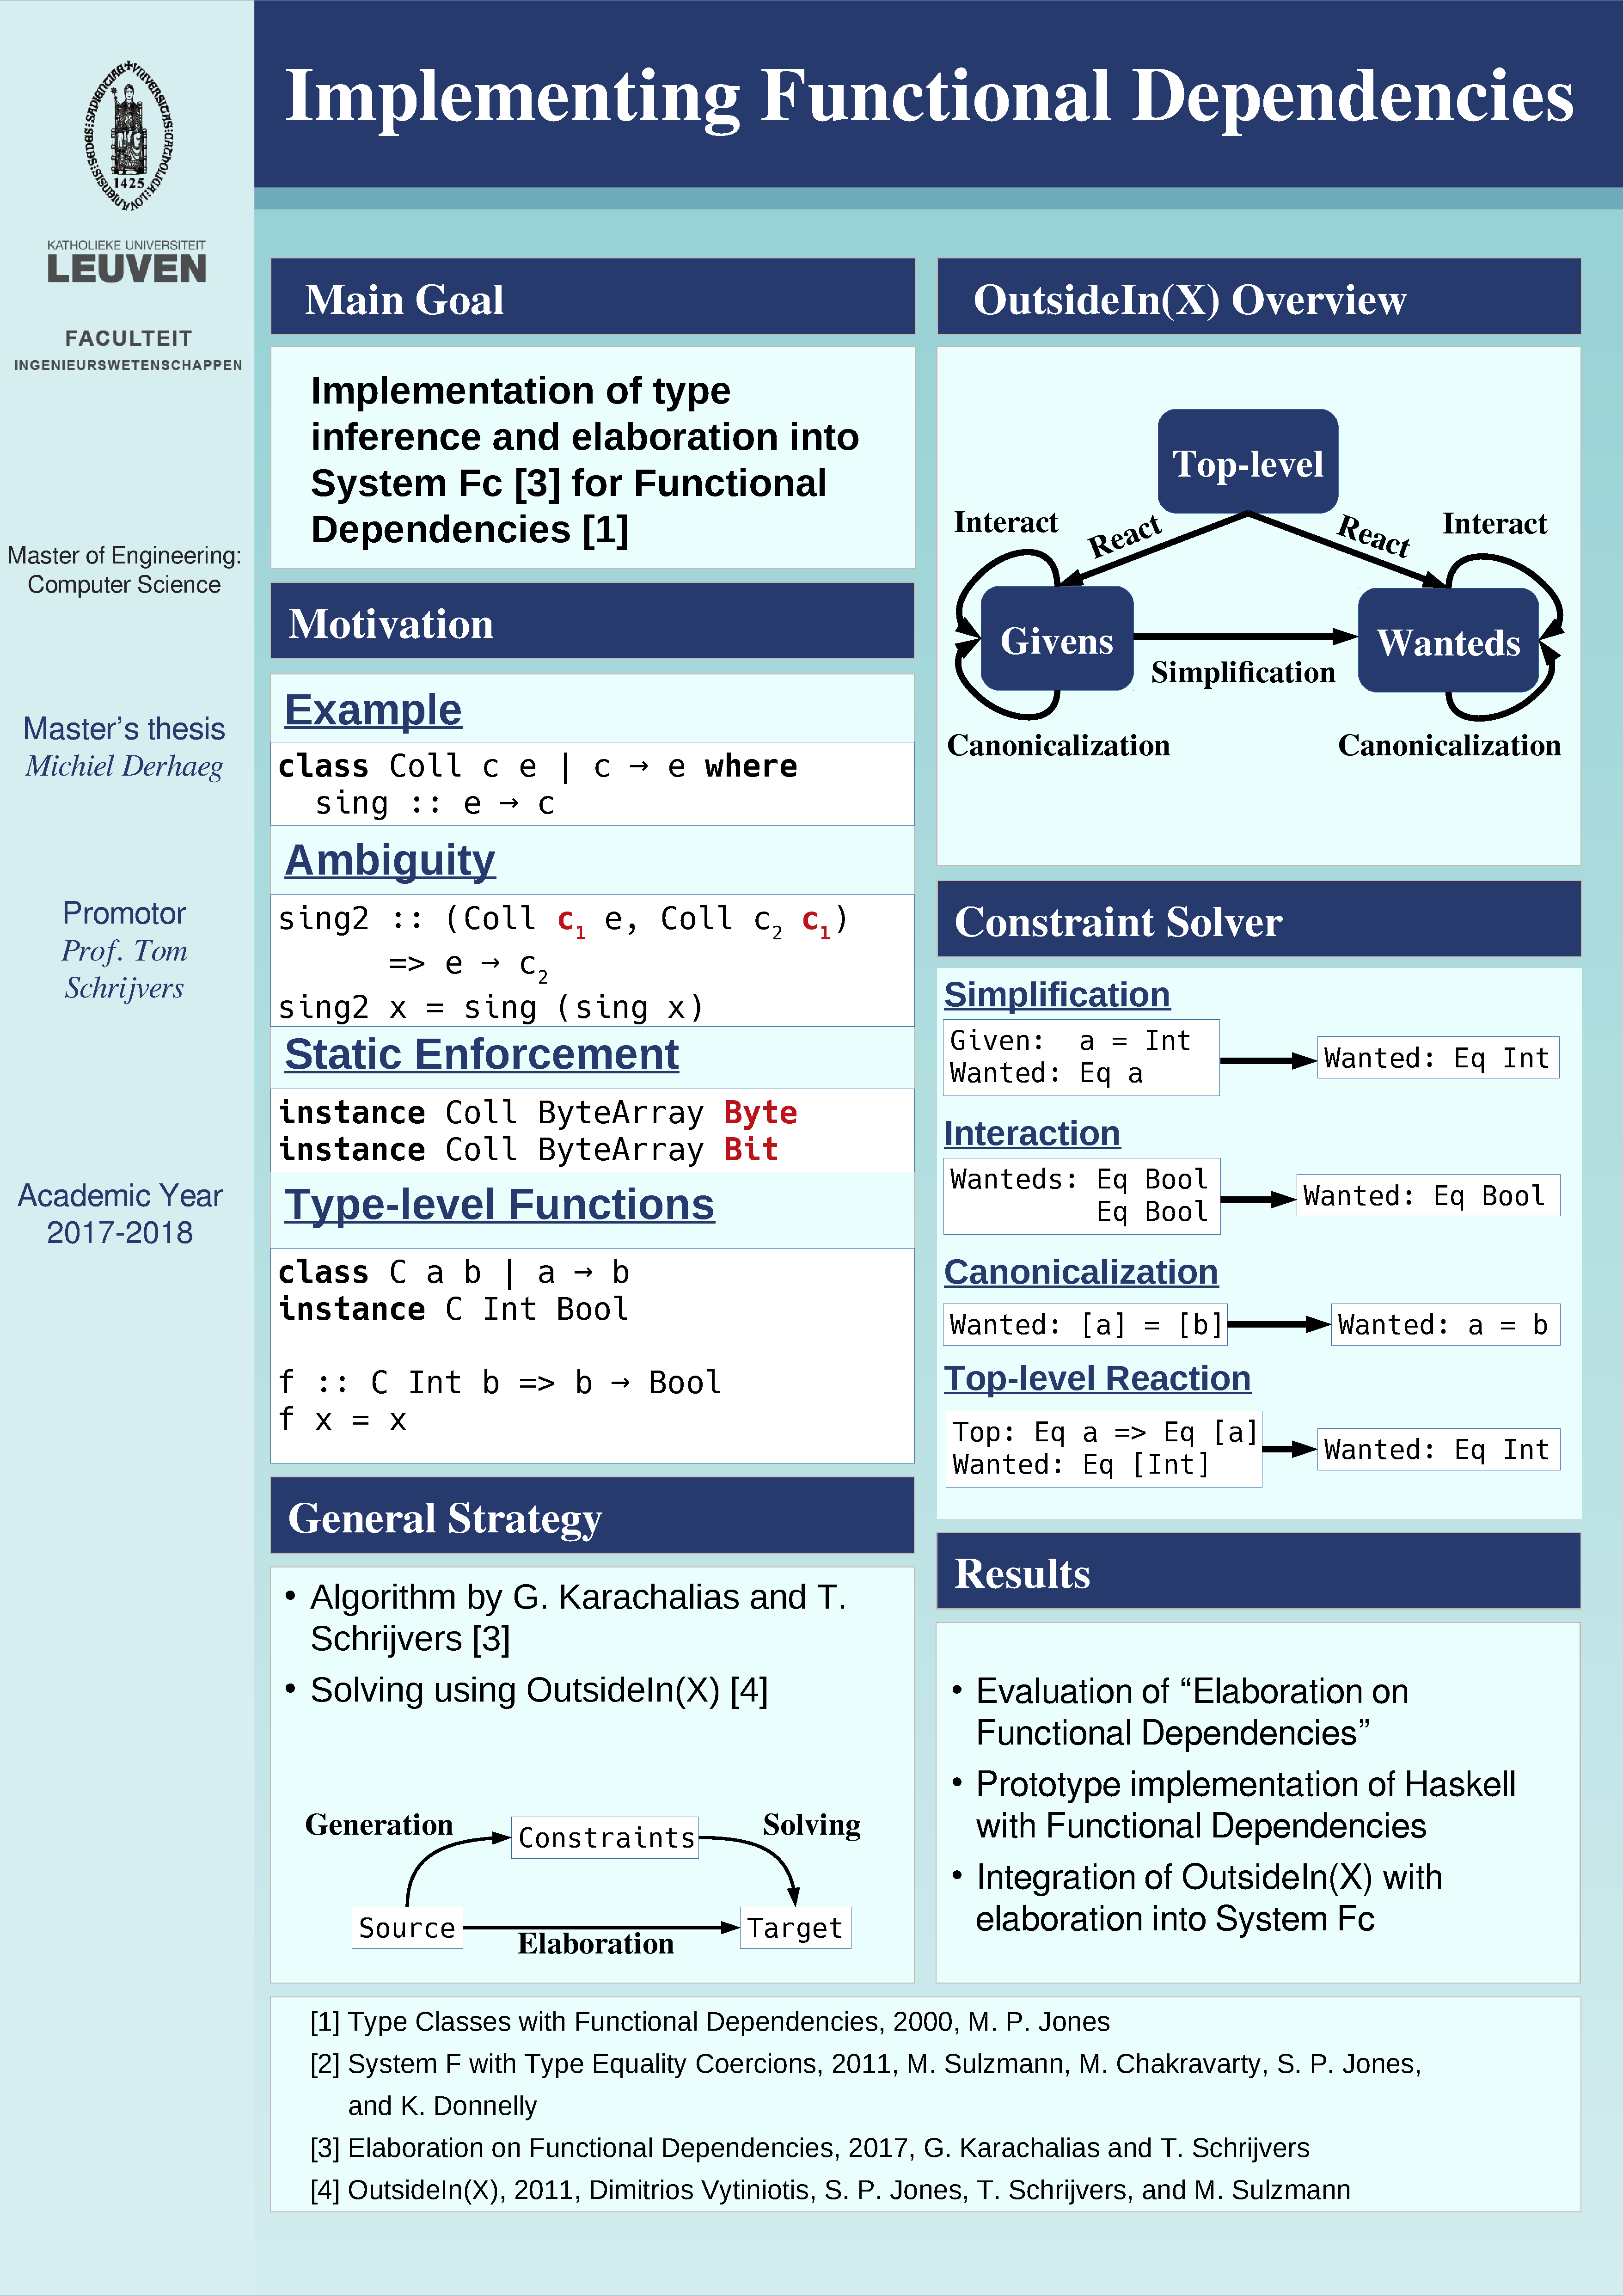
\includepdf[pages=-]{poster.pdf}


\backmatter
\bibliography{references}{}
\bibliographystyle{plain}
\end{document}
